\section{A toy example} 
\begin{frame}{A Naive approach to Permutation Testing}
\bb{Comparison of Two Samples (i.e. one factor with two levels)} 
\bi 
\item[$\cdot$] {\bf Control}: 3 observations,
\item[$\cdot$] \rbf{Treated}: 3 observations:
\ei
$$\gbf{1.025}, \gbf{1.949}, \gbf{3.477}, \rbf{2.391}, \rbf{3.676}, \rbf{4.816}$$
\eb
\bb{Hypothesis testing} 
\bi 
\item $H_0$: Two groups are equal
\item $H_1$: Treated is greater than Control (on average)
\ei
\eb
\rbf{$p$-value}: probability to get the observed evidence against $H_0$ if the two groups were equal (i.e.  $H_0$ were true)\\
\rbf{Test}: if $p\leq\alpha$ (e.g. $\alpha=.05$): we decide for $H_1$,\\\qquad\ \  otherwise: we stay with $H_0$ 
\end{frame}
%%%%%%%%%%%%%%%%%%
\bfr{Parametric approach}
Assumptions on $y_1,y_2,\ldots,y_6$
\bi
\item independent
\item identically distributed
\item[] \bi
  \item normally distributed% $N(\mu_{Treated},\sigma^2)$ and $N(\mu_{Control},\sigma^2)$
  \item[] OR
  \item have finite mean and variance (but inference is only asymptotically valid in this case!)
  \ei
\ei
\pause

We can perform a t-test:
 $$T=\frac{\bar{y}(Treated)-\bar{y}(Control)}
 {\widehat{sd(\bar{y}(Treated)-\bar{y}(Control))}}\sim t_4$$
(i.e. T test statistic follow a $t$ distribution with n-2=4 d.f.)
\end{frame}
%%%%%%%%%%%%%%%%%%
\bfr{Parametric approach}

With toy data:\\
{\tt t = -1.4545, \\
df = 4,\\
p-value = 0.1098}
\bigskip

\bb{Remark}
The hypotheses tested are:
\bi
\item $H_0: \mu_{Treated}=\mu_{Control}$
\item $H_1: \mu_{Treated}>\mu_{Control}$ (only a difference in mean is allowed)
\ei
\eb
\end{frame}
%%%%%%%%%%%%%%%%%%%%%
\section{A Naive approach to Permutation Testing}
\bfr{A Naive approach to Permutation Testing}
The $p$-value is computed \bbf{under $H_0$:} \\
\gbf{Controls} and \rbf{Treated} have the \bbf{same distribution}.
\bigskip

\bb{Collection of equally likely outcomes:}
\begin{eqnarray*}
&&f(\gbf{1.025}, \gbf{1.949}, \gbf{3.477}, \rbf{2.391}, \rbf{3.676}, \rbf{4.816}) =\\ \pause
&=&f(\gbf{1.025}, \rbf{1.949}, \gbf{3.477}, \rbf{2.391}, \gbf{3.676}, \rbf{4.816})=\\ \pause
&=&f(\rbf{1.025}, \rbf{1.949}, \gbf{3.477}, \gbf{2.391}, \rbf{3.676}, \gbf{4.816})=\\ \pause
&=& \ldots
\end{eqnarray*}
\eb

There are ${6 \choose 3}=\frac{6!}{3!3!}=20$ equally likely outcomes

\end{frame}

\bfr{A Naive approach to Permutation Testing}
Compute the difference in mean of the two samples
\begin{center}
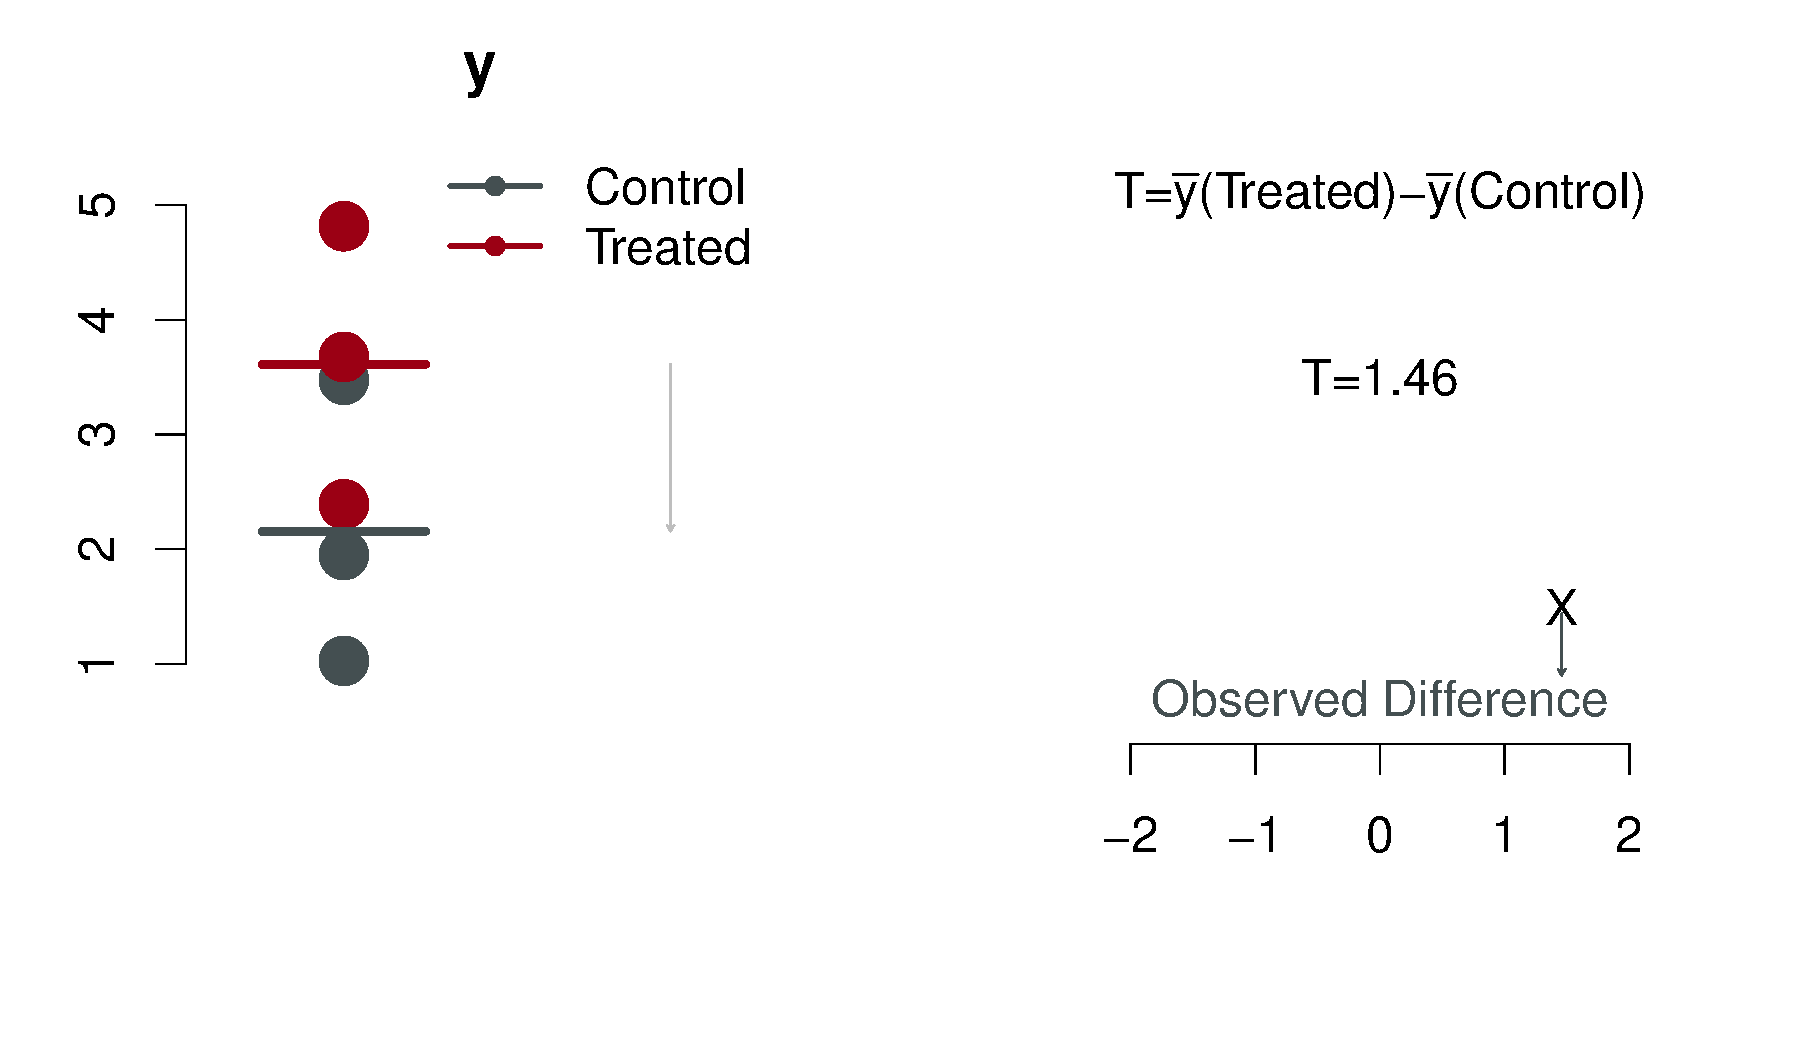
\includegraphics[width=1.1\textwidth]{figures/permsslides1} 
\end{center}
\end{frame}


\bfr{A Naive approach to Permutation Testing}
Compute the same difference on another hypothetical experiment
\begin{center}
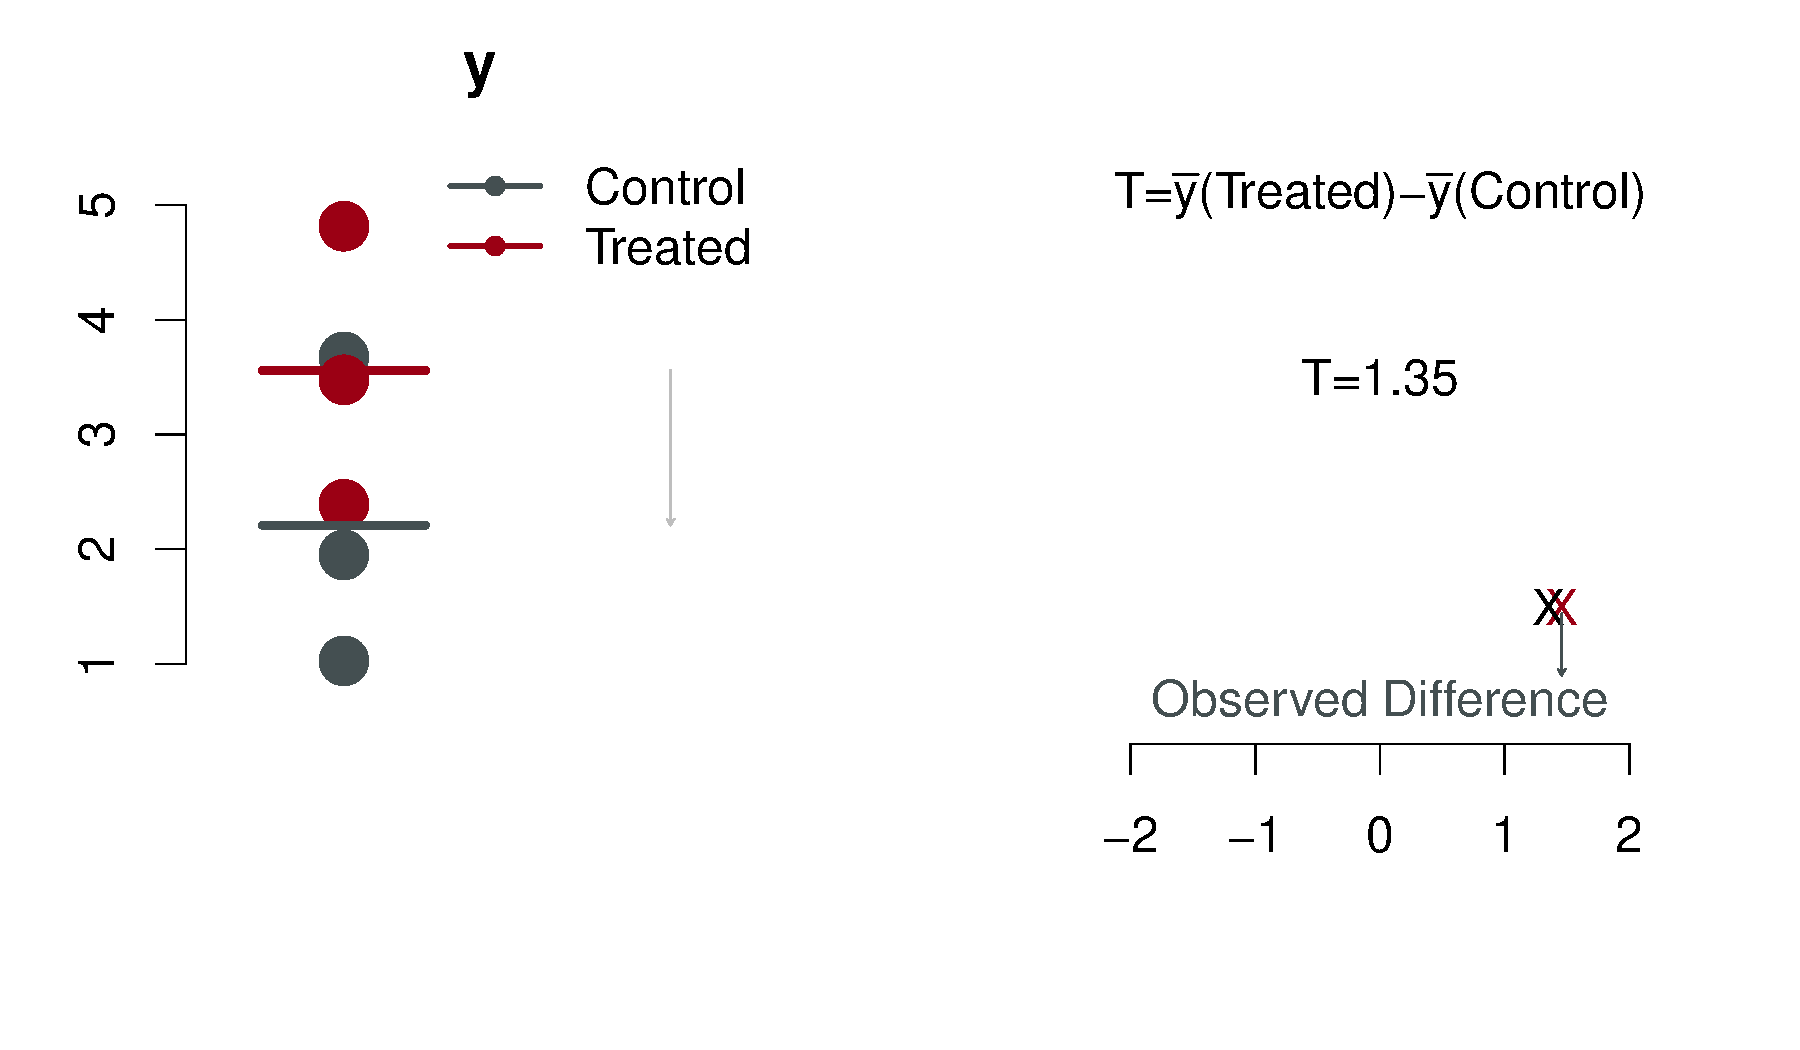
\includegraphics[width=1.1\textwidth]{figures/permsslides2} 
\end{center}
\end{frame}


\begin{frame}{A Naive approach to Permutation Testing}
\ldots and go on with all hypothetical experiments\ldots
\begin{center}
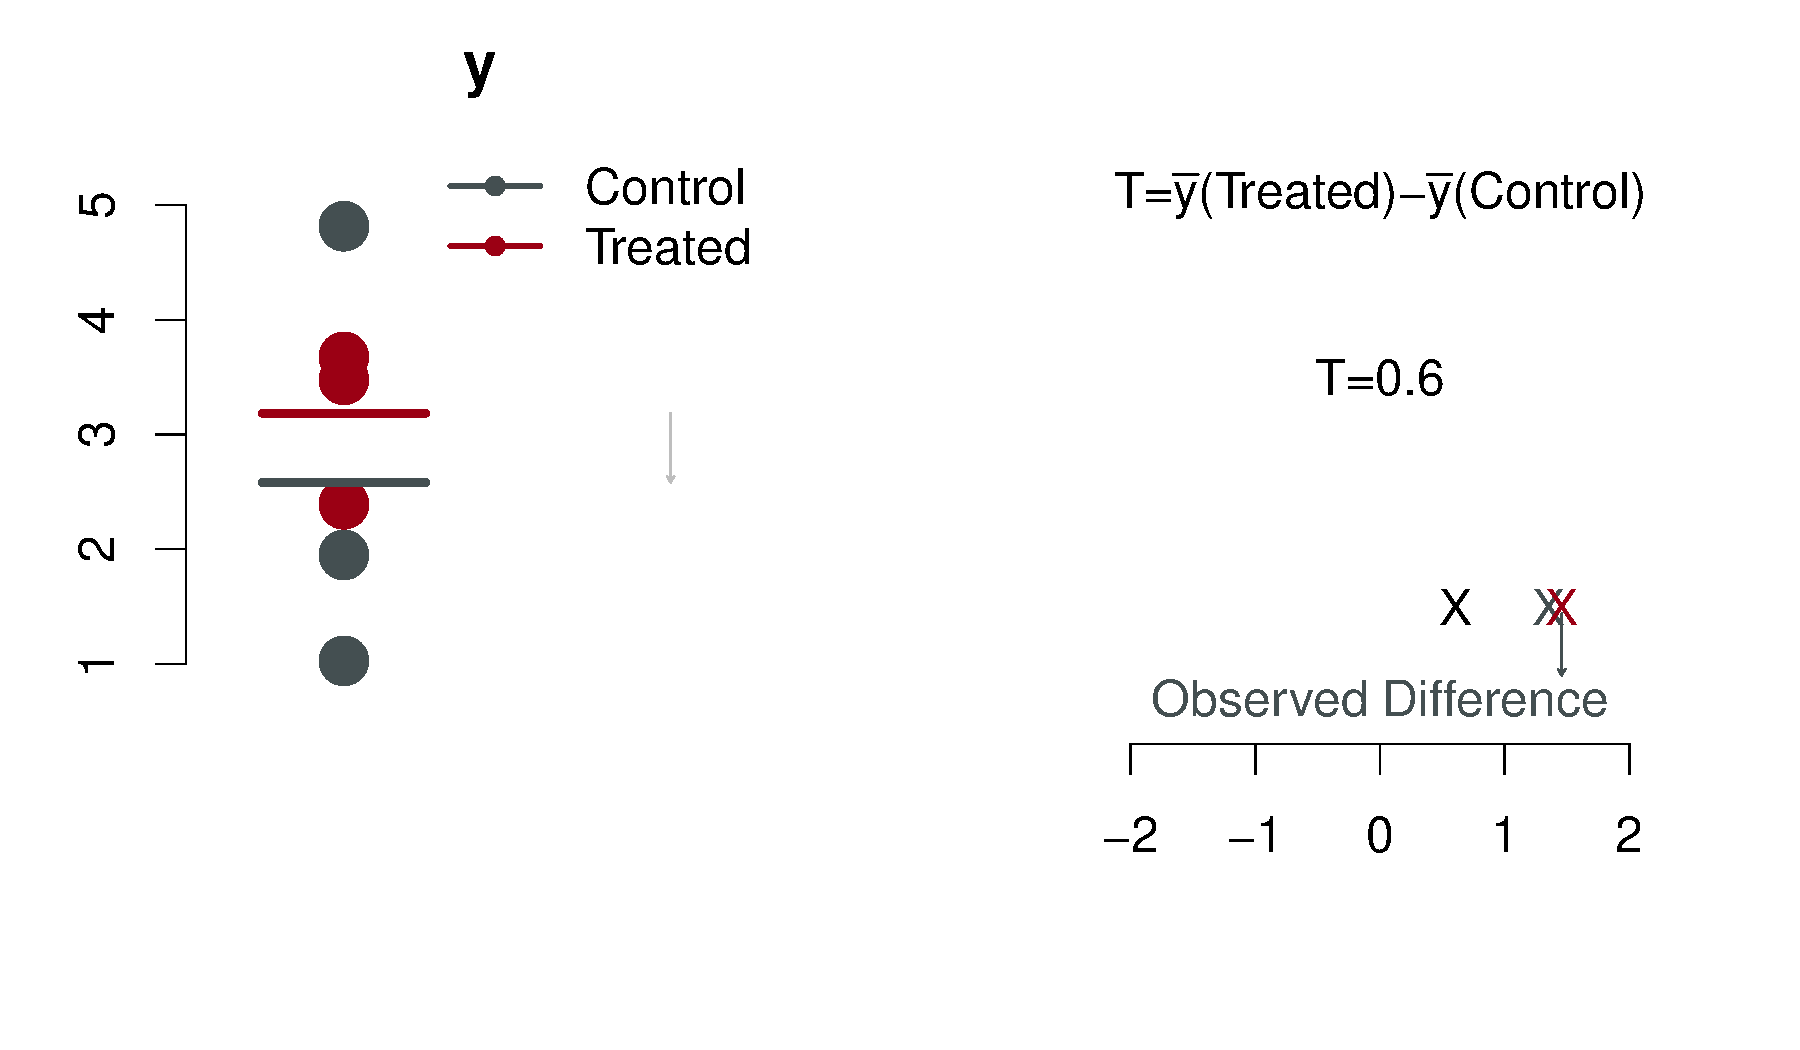
\includegraphics[width=1.1\textwidth]{figures/permsslides3} 
\end{center}
\end{frame}


\begin{frame}{A Naive approach to Permutation Testing} 
\ldots and go on with all hypothetical experiments\ldots
\begin{center}
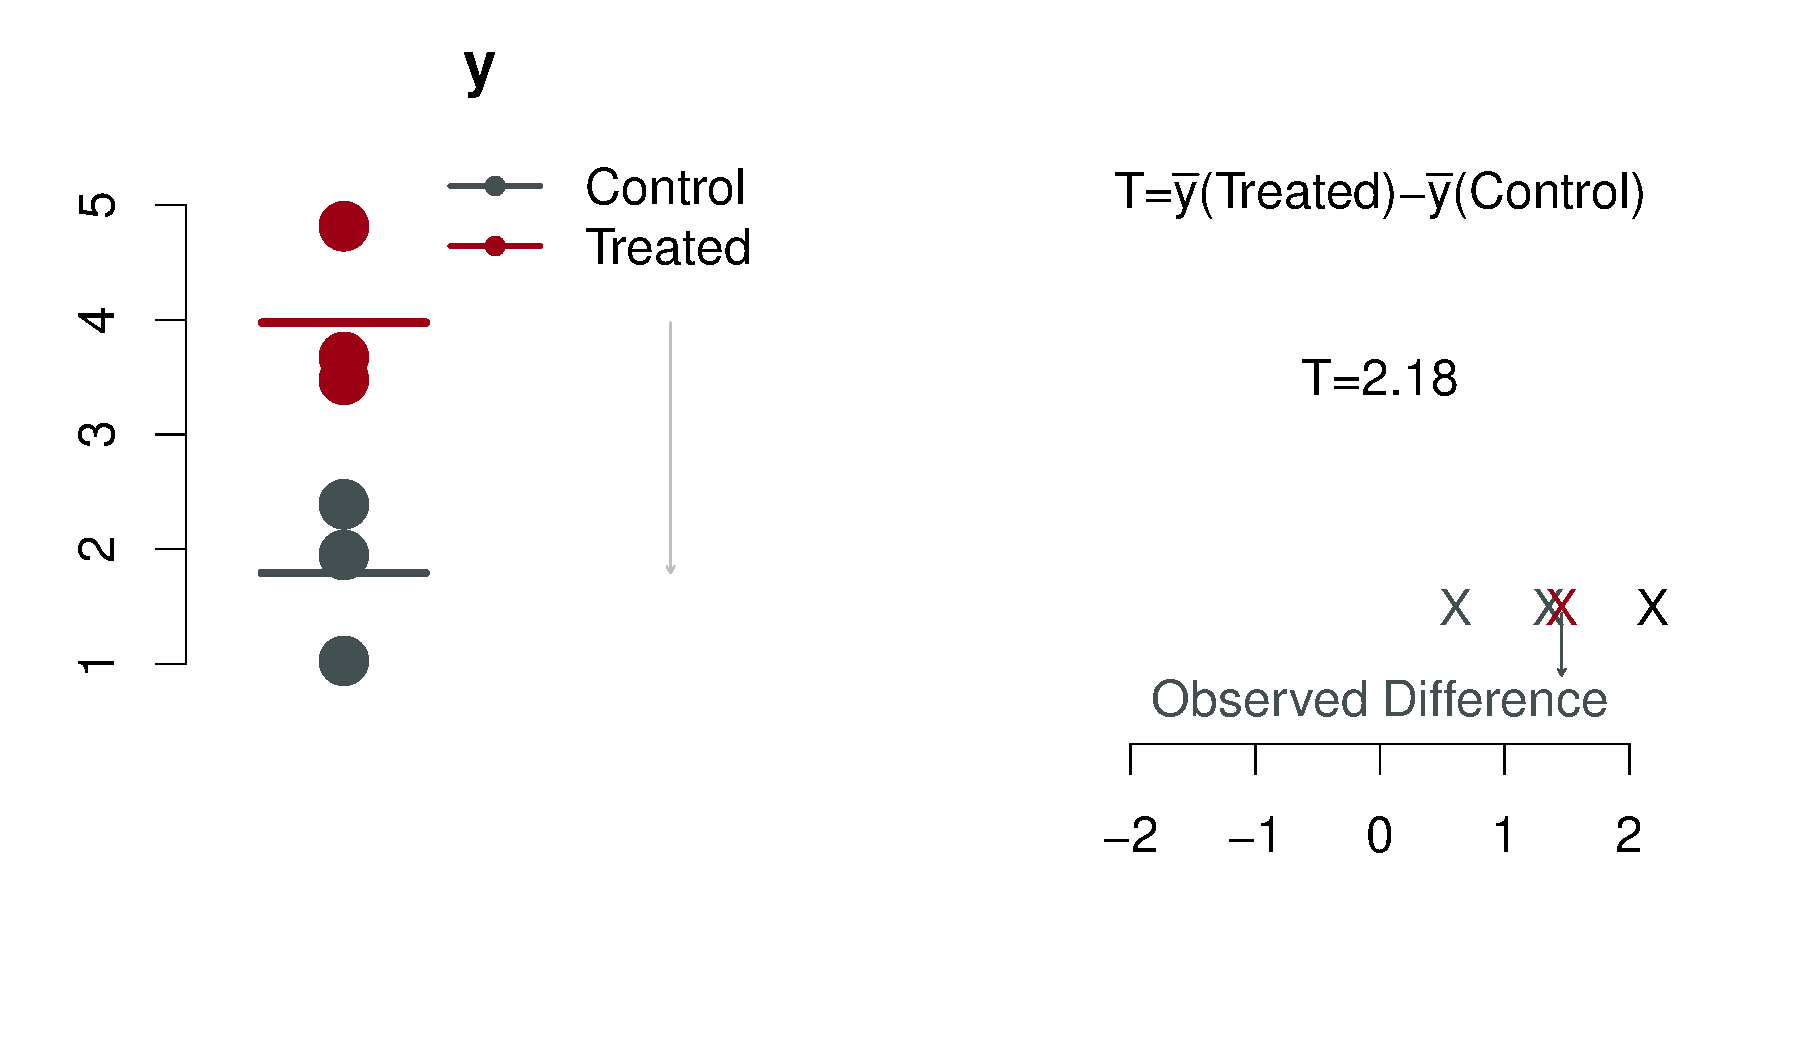
\includegraphics[width=1.1\textwidth]{figures/permsslides4} 
\end{center}
\end{frame}



\begin{frame}{A Naive approach to Permutation Testing} 
\ldots and go on with all hypothetical experiments\ldots
\begin{center}
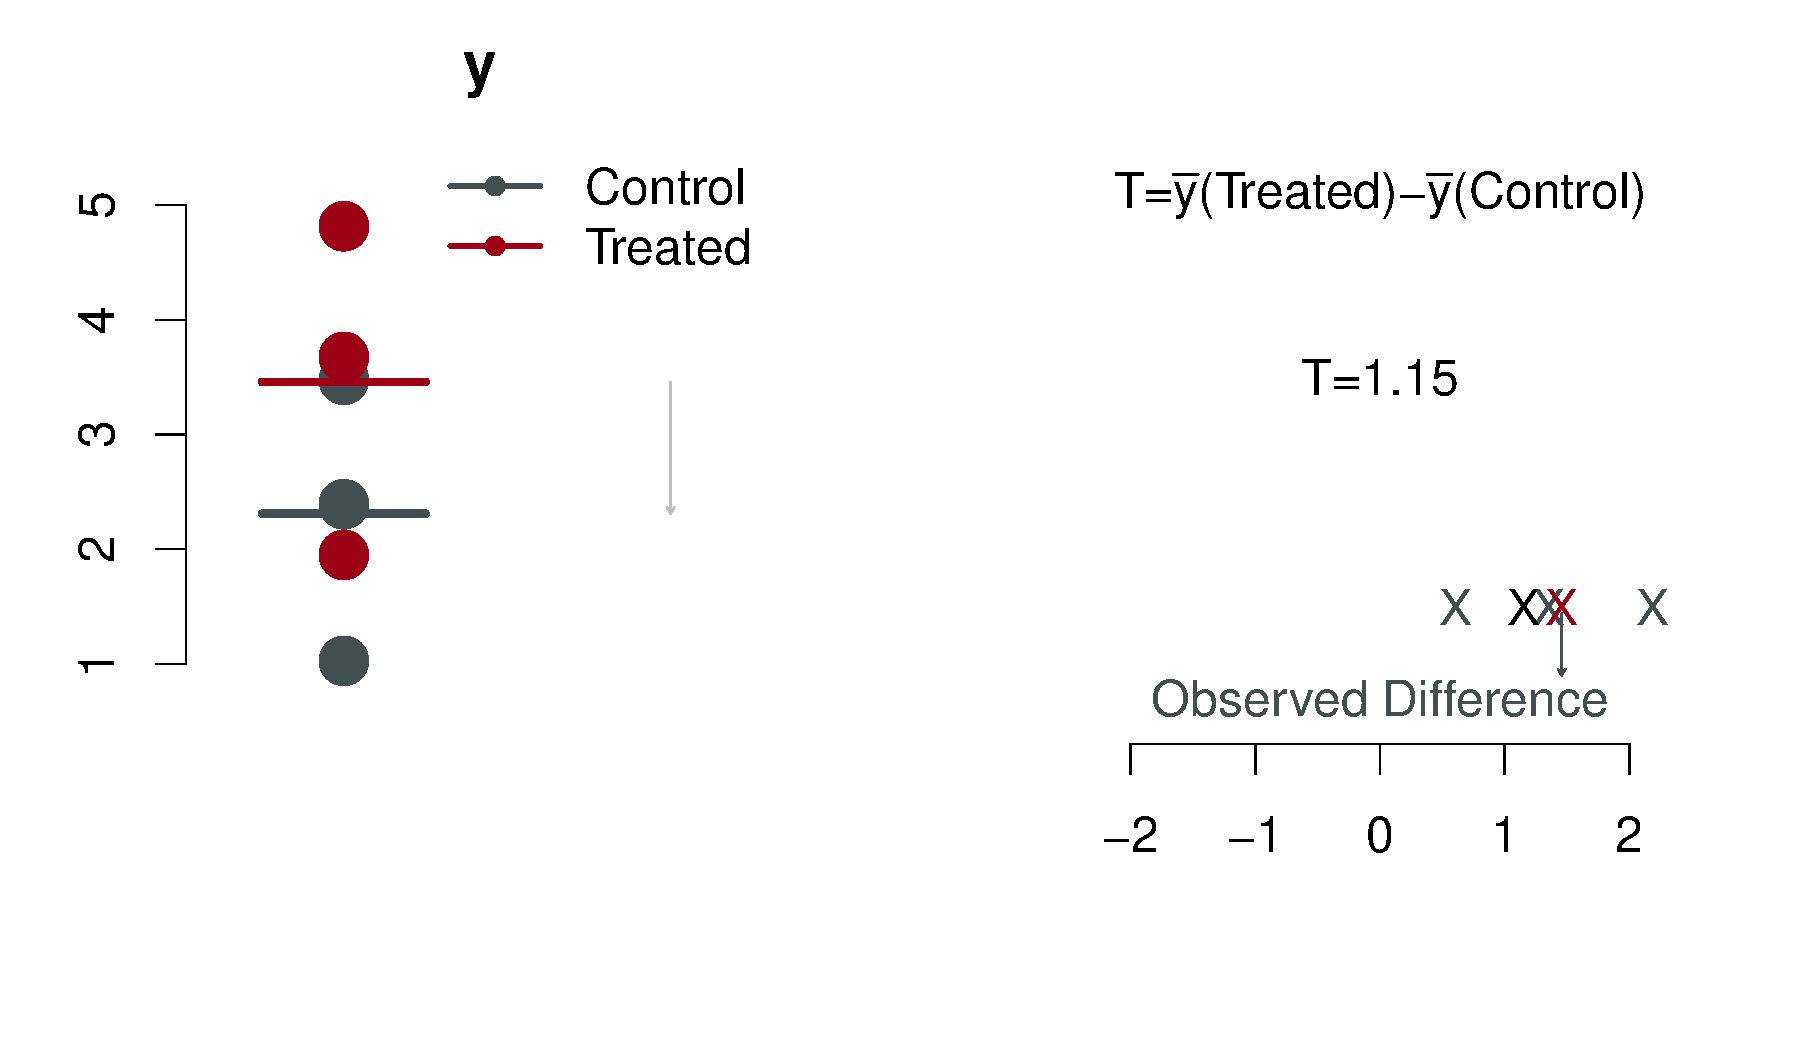
\includegraphics[width=1.1\textwidth]{figures/permsslides5} 
\end{center}
\end{frame}


\begin{frame}{A Naive approach to Permutation Testing}
\ldots and go on with all hypothetical experiments\ldots
\begin{center}
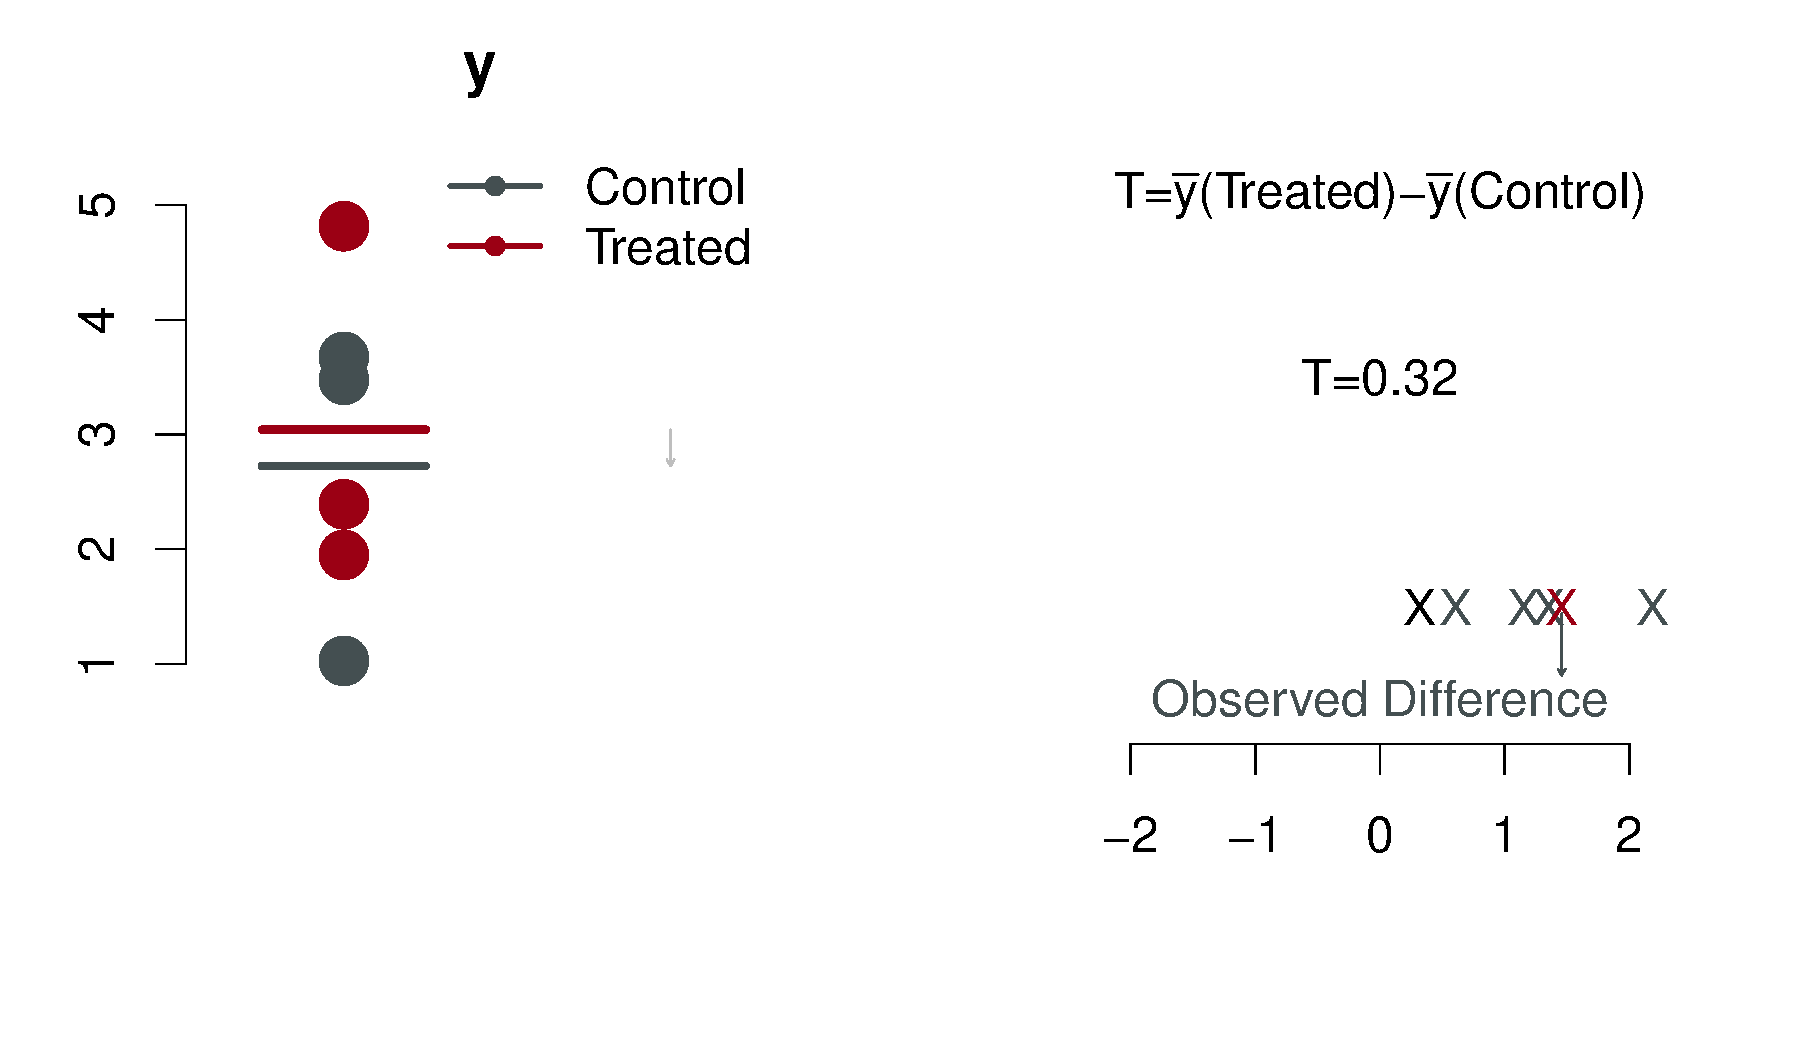
\includegraphics[width=1.1\textwidth]{figures/permsslides6} 
\end{center}
\end{frame}


\begin{frame}{A Naive approach to Permutation Testing}
\ldots and go on with all hypothetical experiments\ldots
\begin{center}
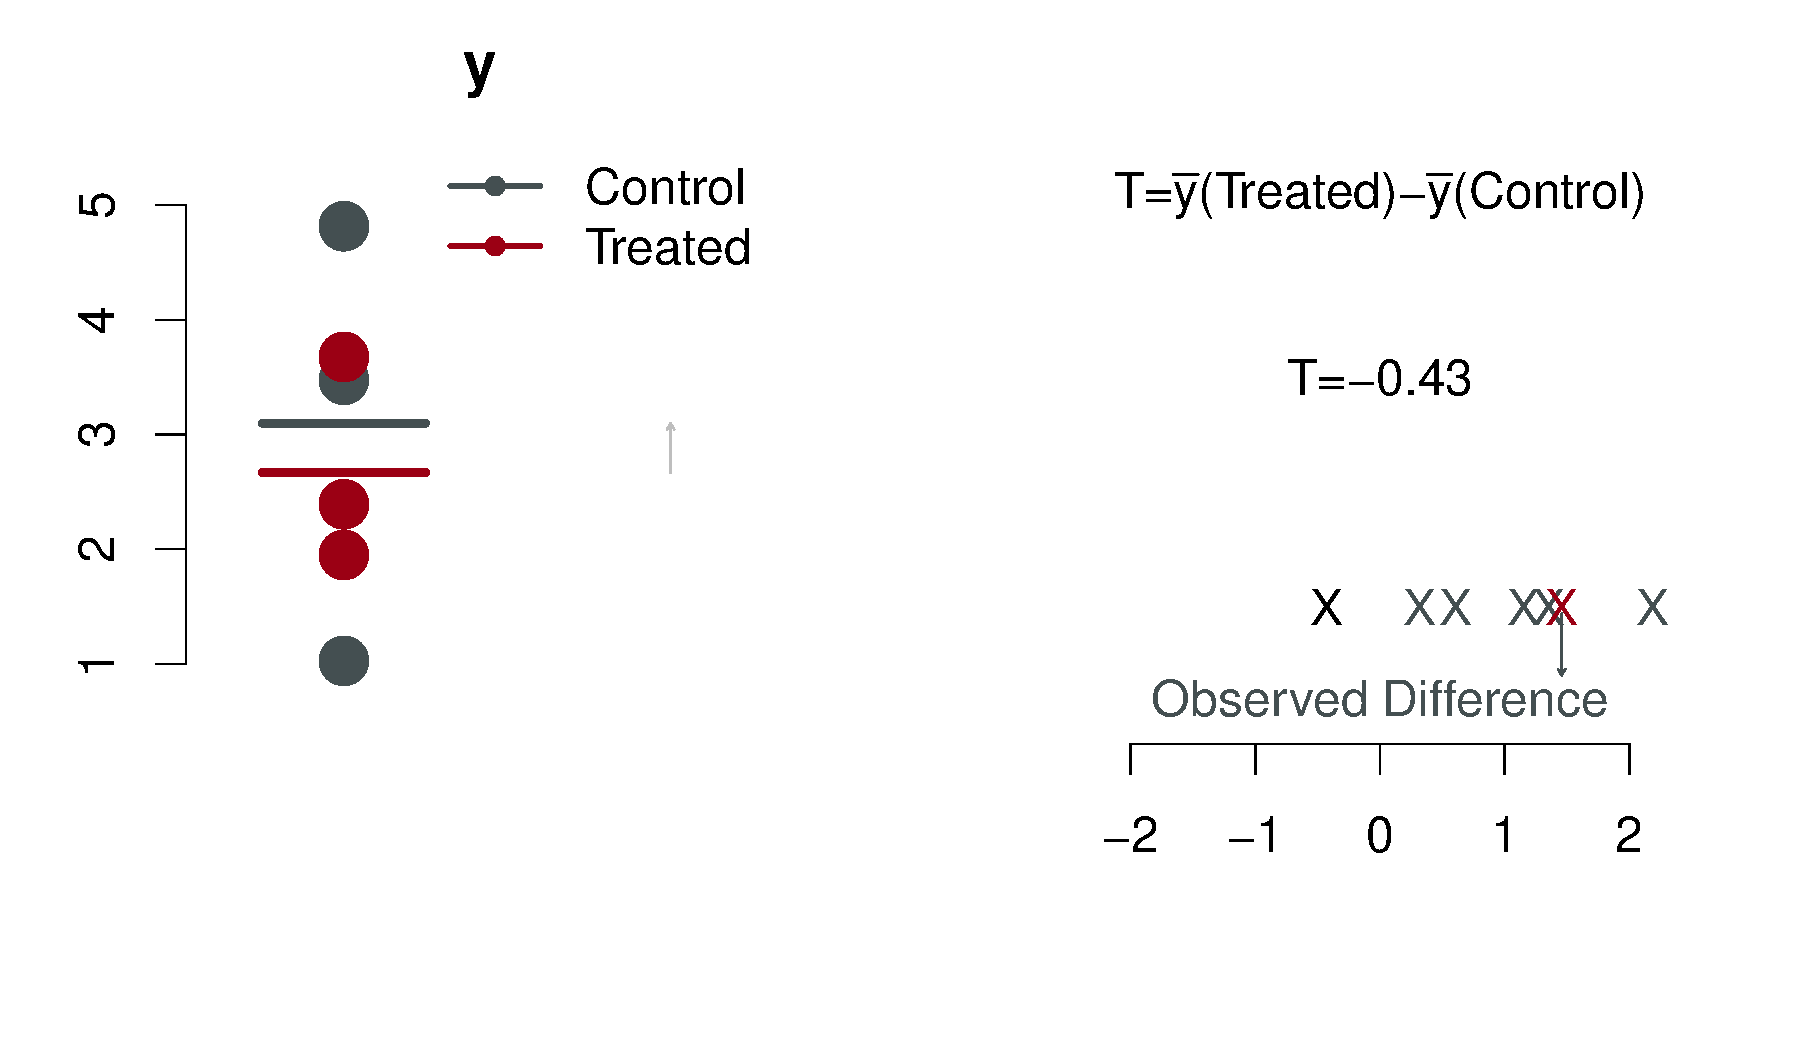
\includegraphics[width=1.1\textwidth]{figures/permsslides7} 
\end{center}
\end{frame}



\begin{frame}{A Naive approach to Permutation Testing}
\ldots and go on with all hypothetical experiments\ldots
\begin{center}
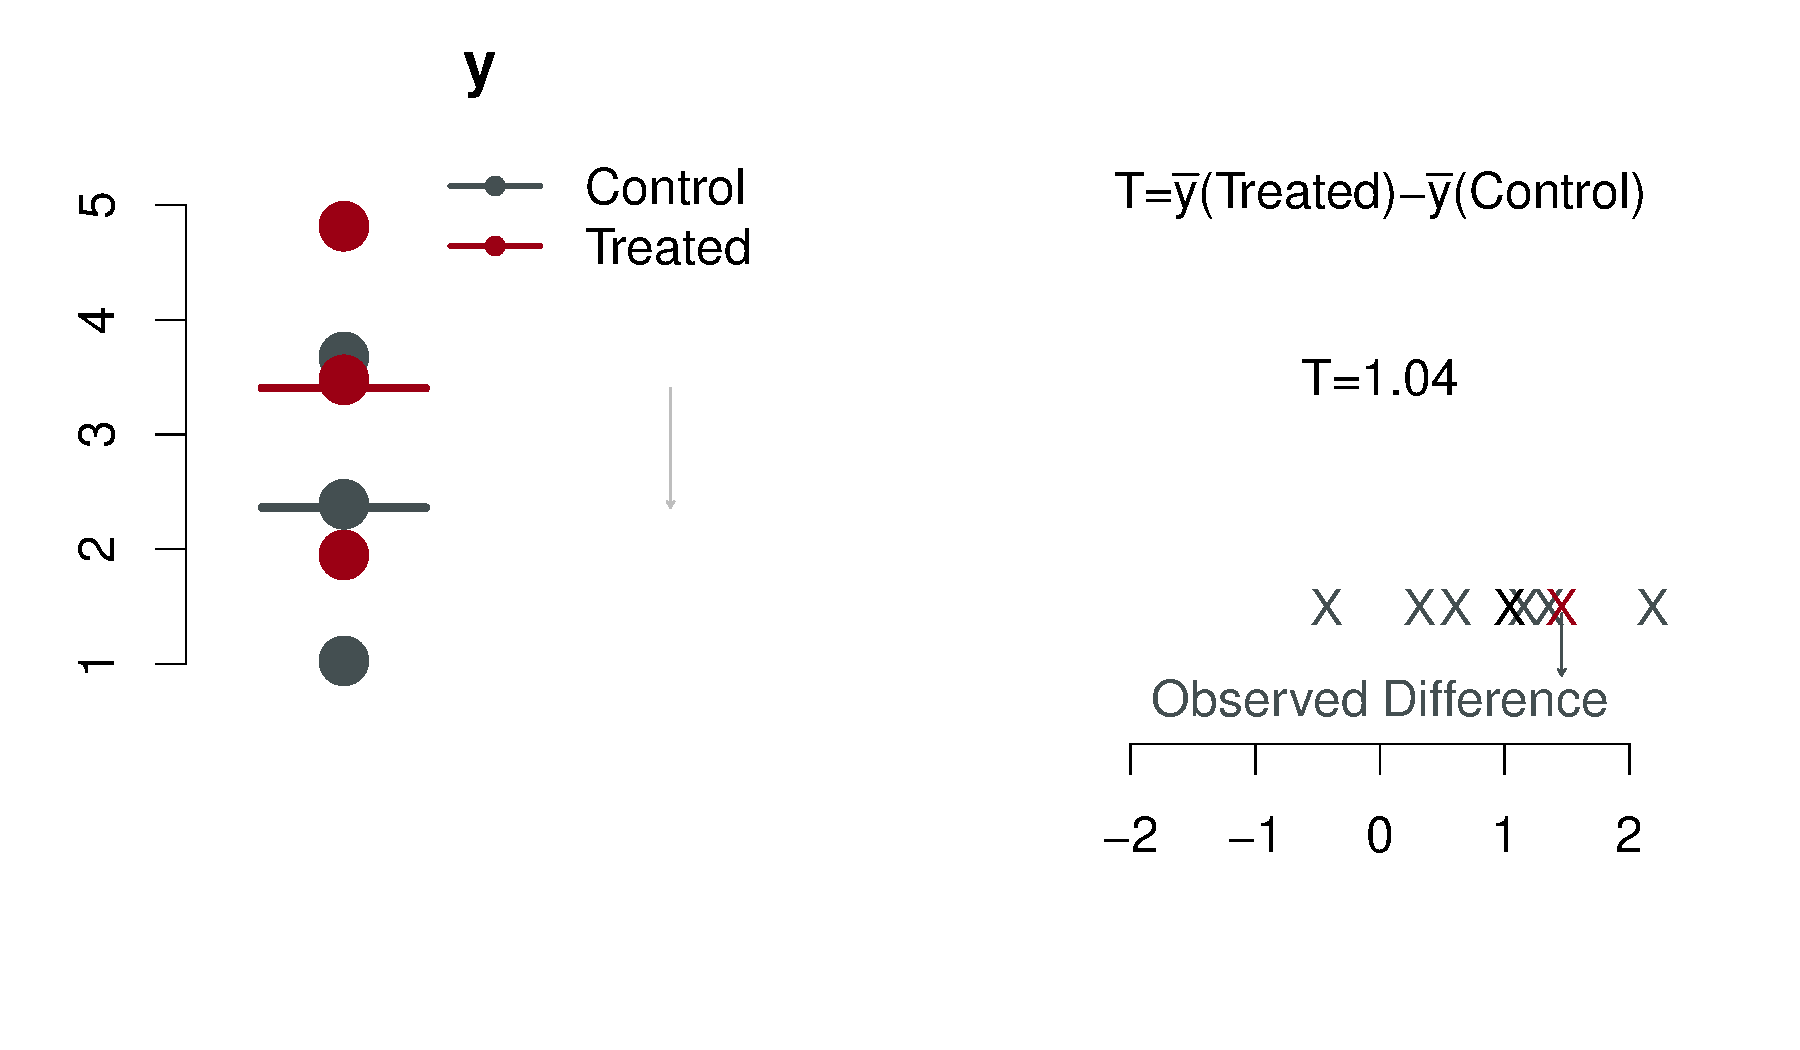
\includegraphics[width=1.1\textwidth]{figures/permsslides8} 
\end{center}
\end{frame}


\begin{frame}{A Naive approach to Permutation Testing} 
\ldots and go on with all hypothetical experiments\ldots
\begin{center}
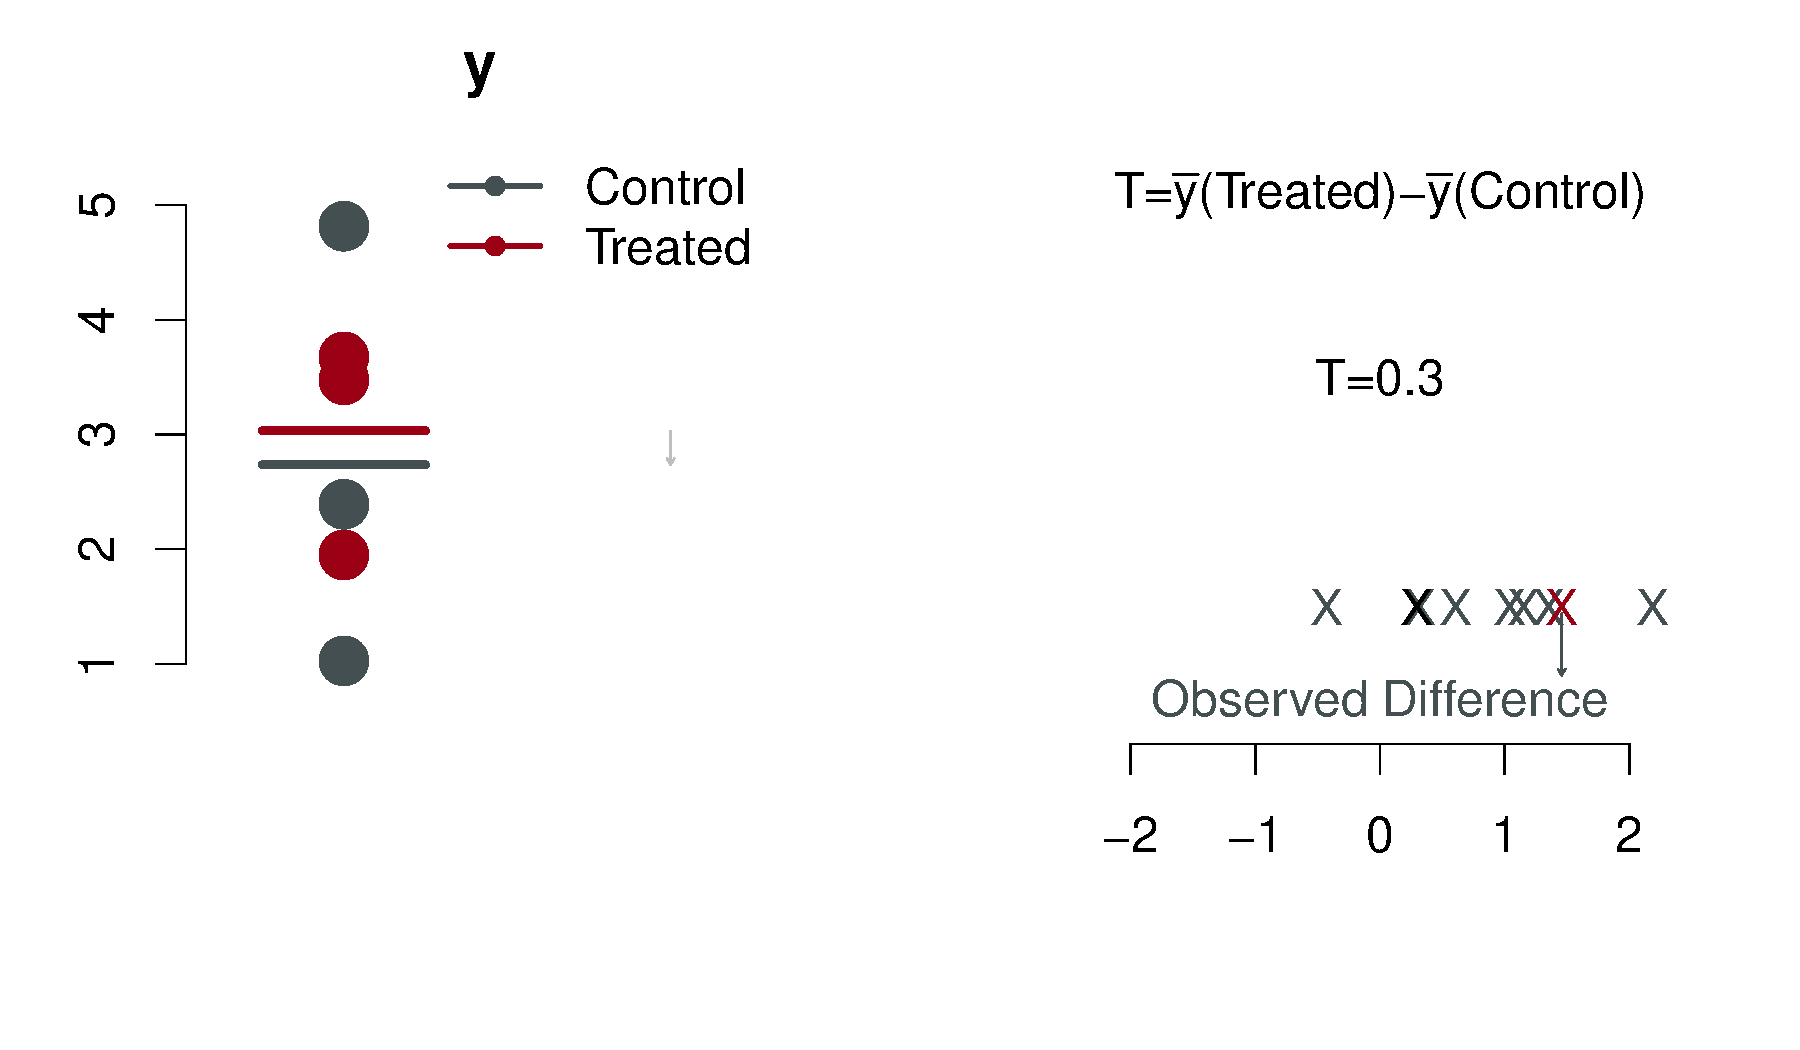
\includegraphics[width=1.1\textwidth]{figures/permsslides9} 
\end{center}
\end{frame}


\begin{frame}{A Naive approach to Permutation Testing}
\ldots and go on with all hypothetical experiments\ldots
\begin{center}
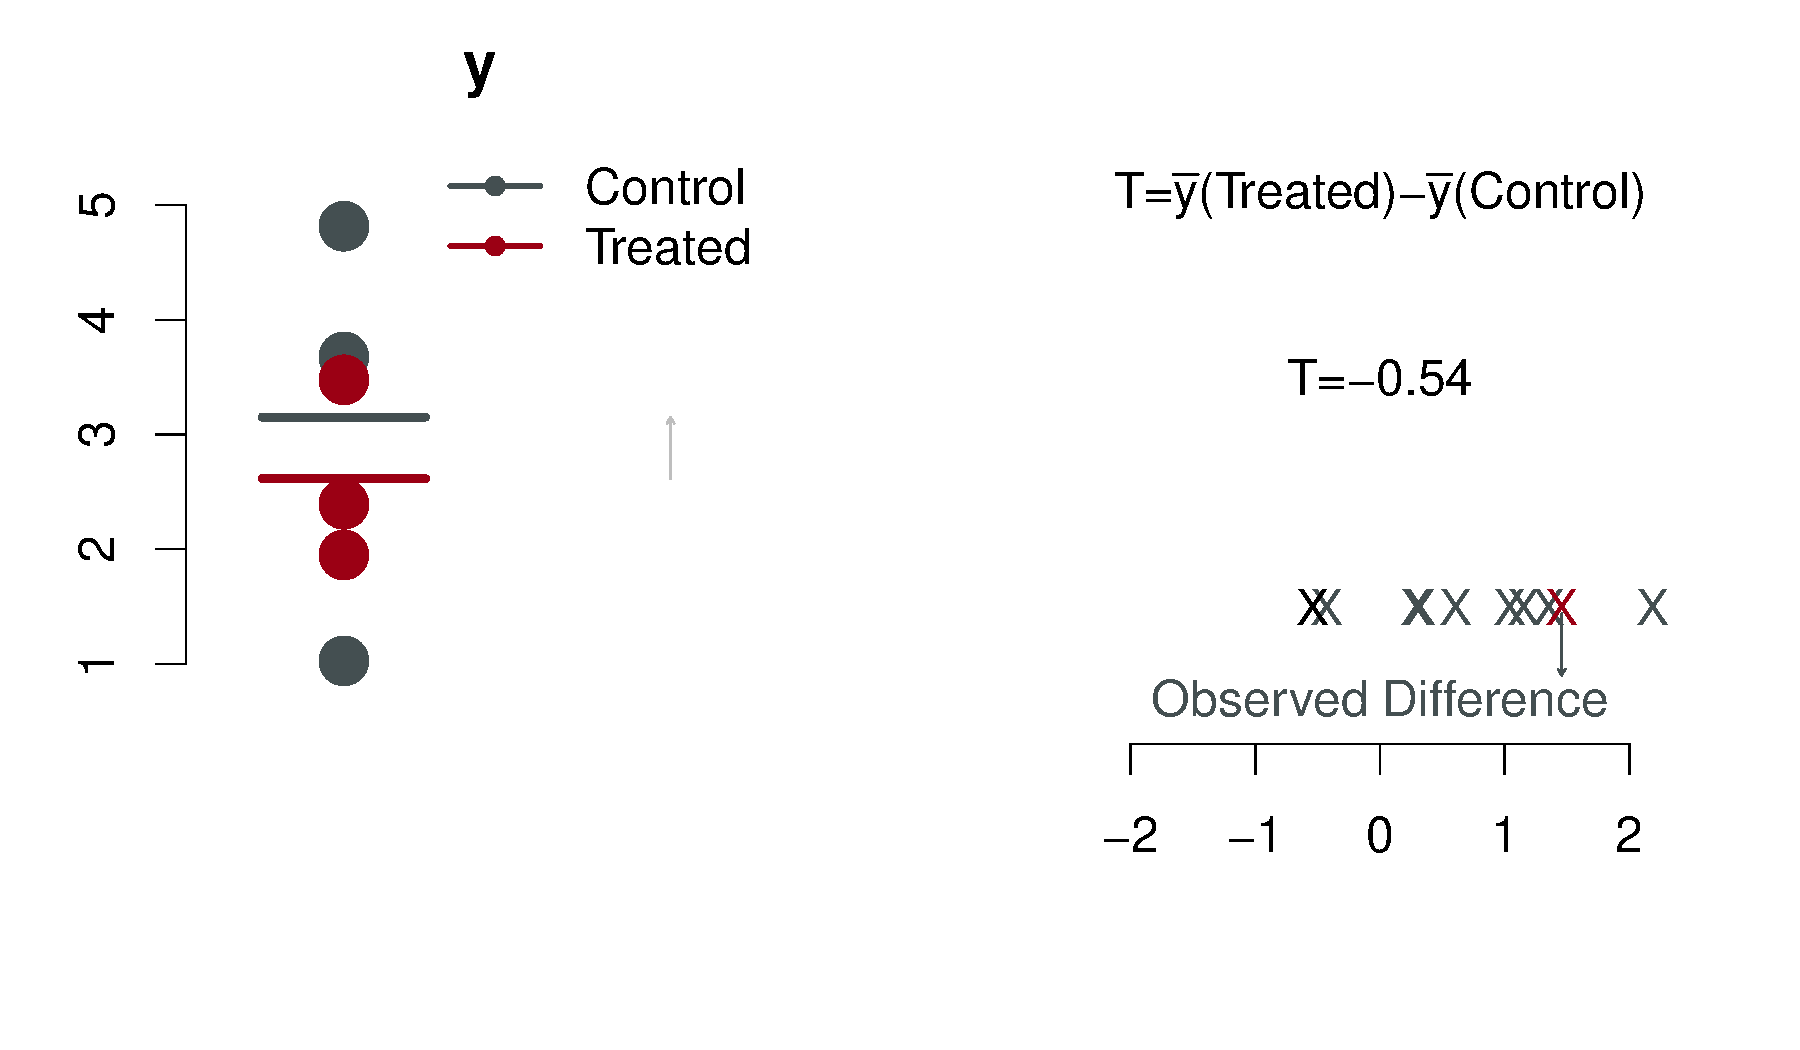
\includegraphics[width=1.1\textwidth]{figures/permsslides10} 
\end{center}
\end{frame}


\begin{frame}{A Naive approach to Permutation Testing}
 \ldots and go on with all hypothetical experiments\ldots 
\begin{center}
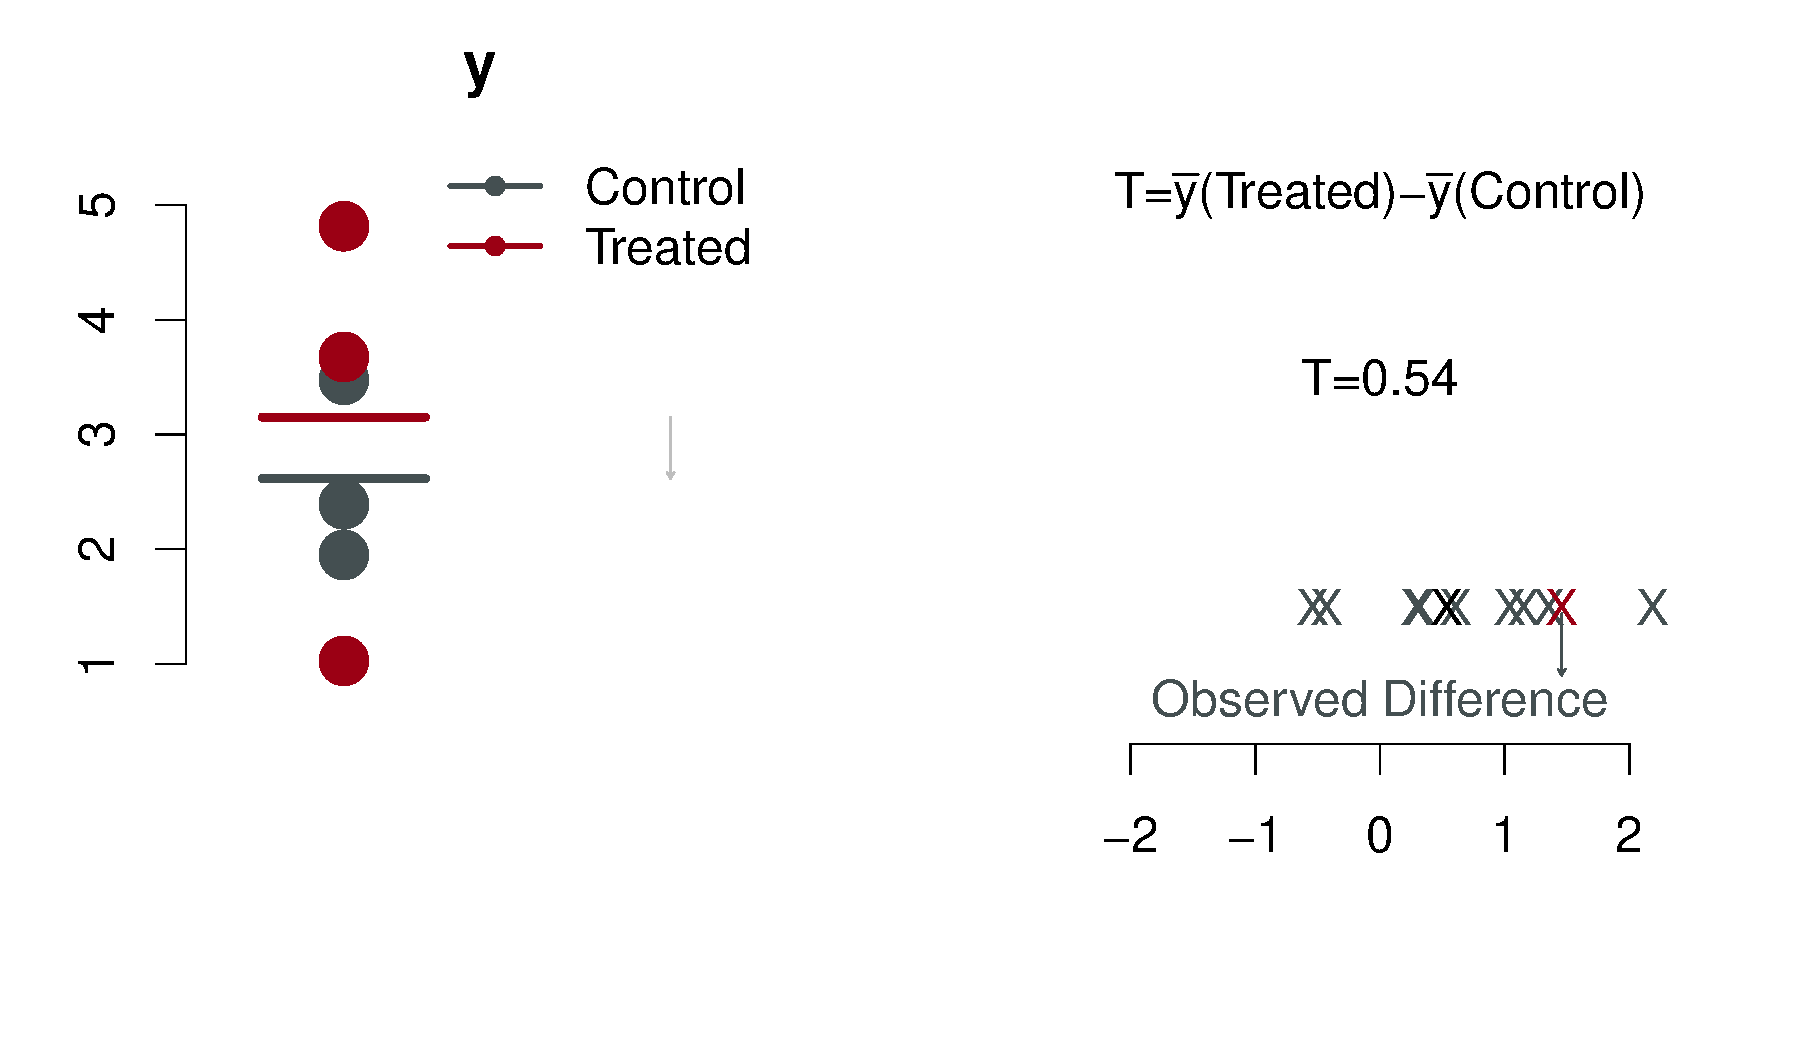
\includegraphics[width=1.1\textwidth]{figures/permsslides11} 
\end{center}
\end{frame}


\begin{frame}{A Naive approach to Permutation Testing}
 \ldots and go on with all hypothetical experiments\ldots 
\begin{center}
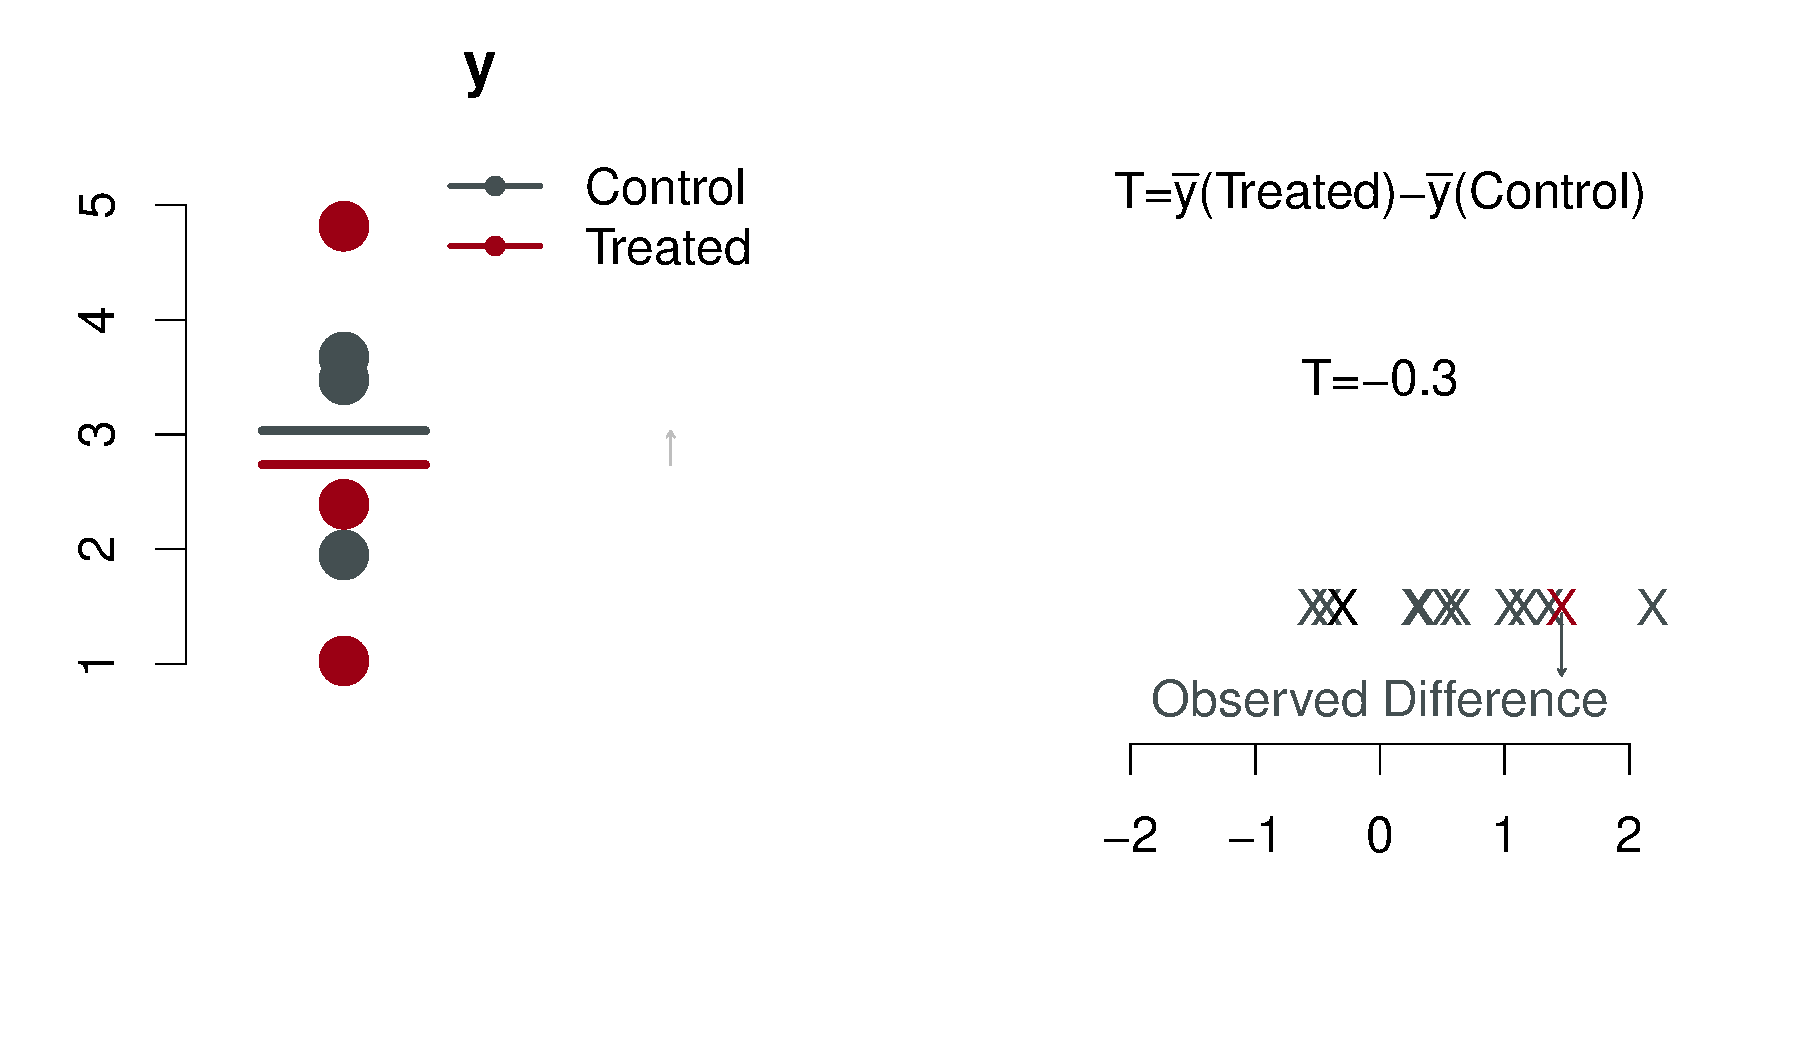
\includegraphics[width=1.1\textwidth]{figures/permsslides12} 
\end{center}
\end{frame}


\begin{frame}{A Naive approach to Permutation Testing}
 \ldots and go on with all hypothetical experiments\ldots 
\begin{center}
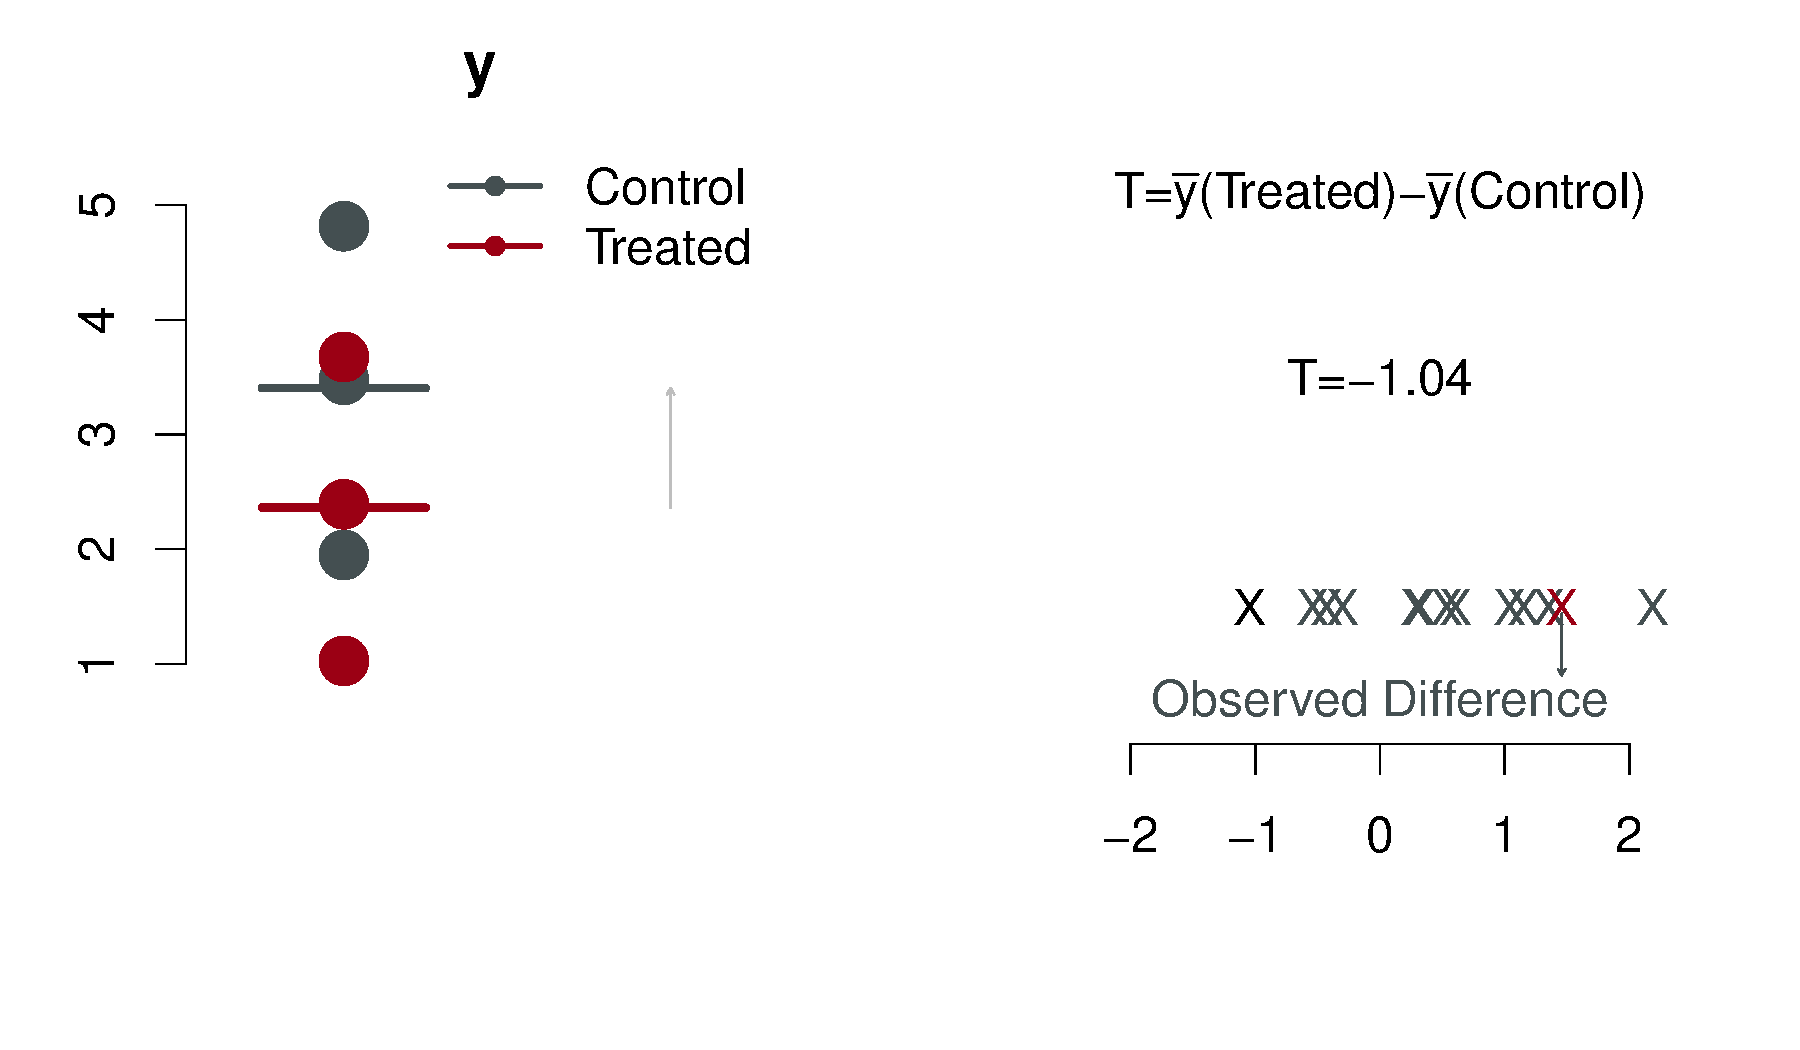
\includegraphics[width=1.1\textwidth]{figures/permsslides13} 
\end{center}
\end{frame}


\begin{frame}{A Naive approach to Permutation Testing}
 \ldots and go on with all hypothetical experiments\ldots 
\begin{center}
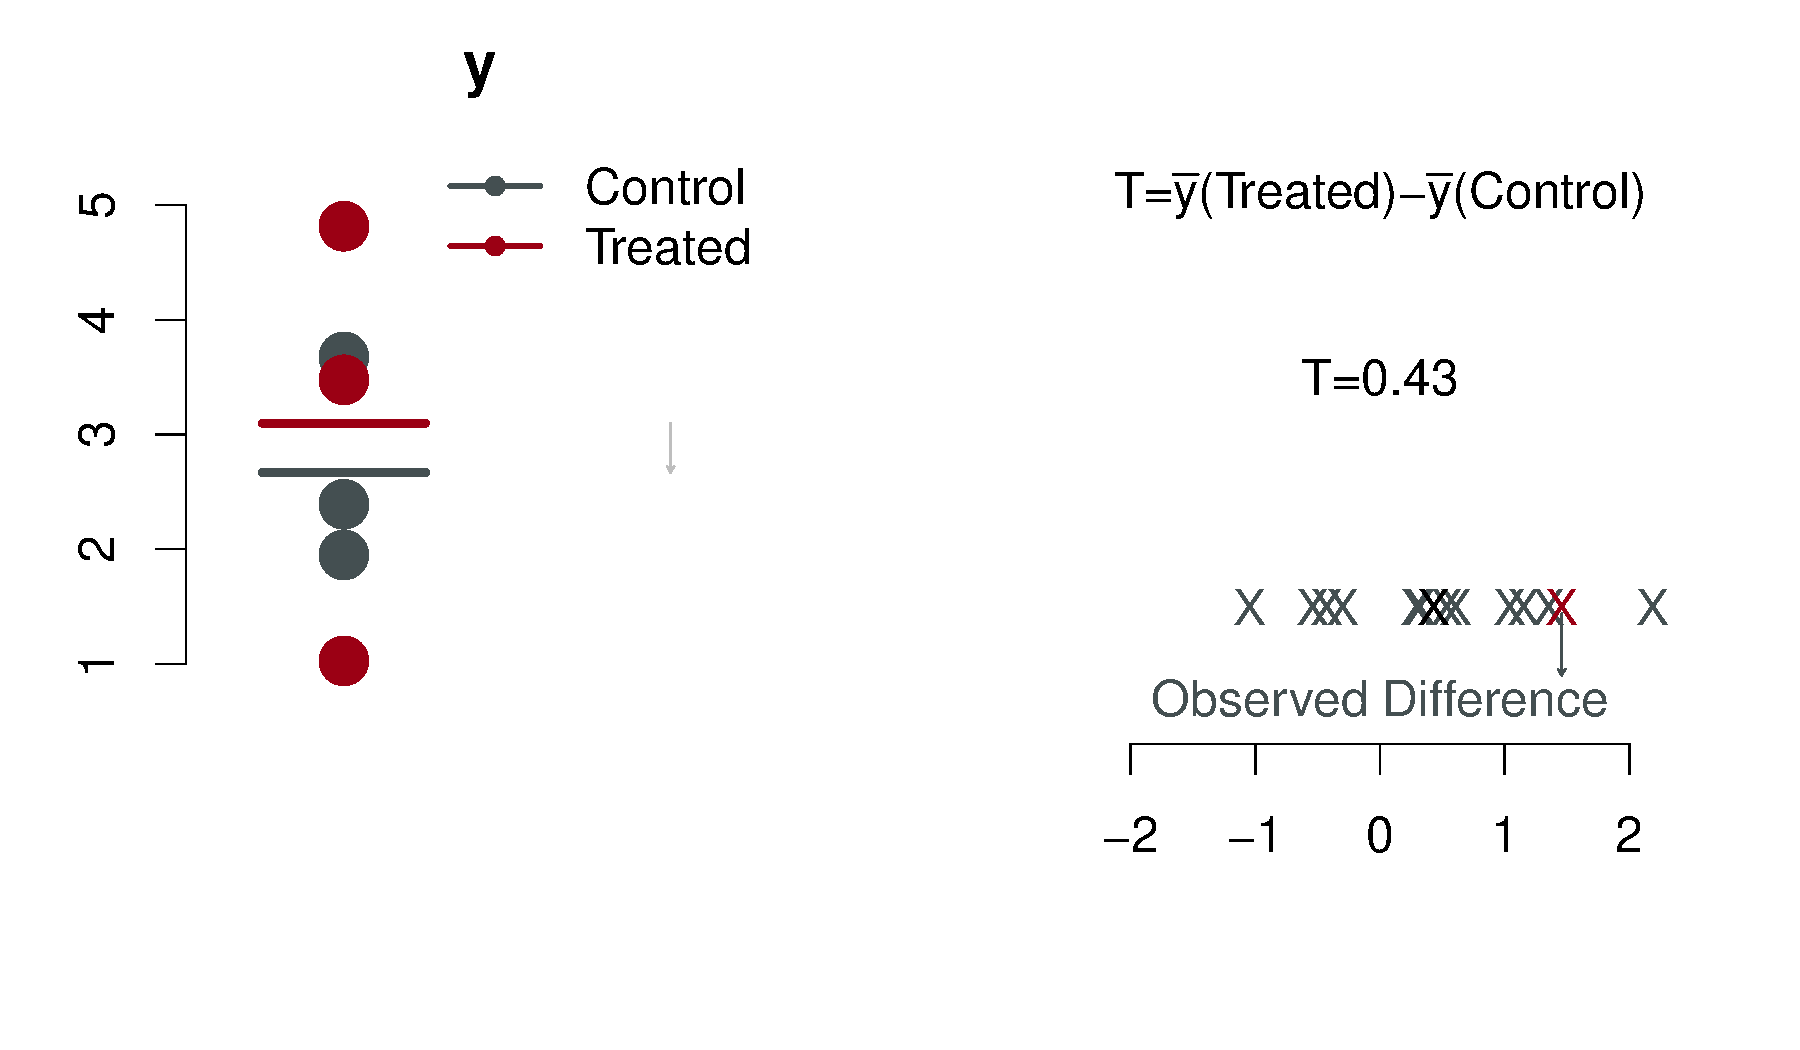
\includegraphics[width=1.1\textwidth]{figures/permsslides14} 
\end{center}
\end{frame}


\begin{frame}{A Naive approach to Permutation Testing}
 \ldots and go on with all hypothetical experiments\ldots 
\begin{center}
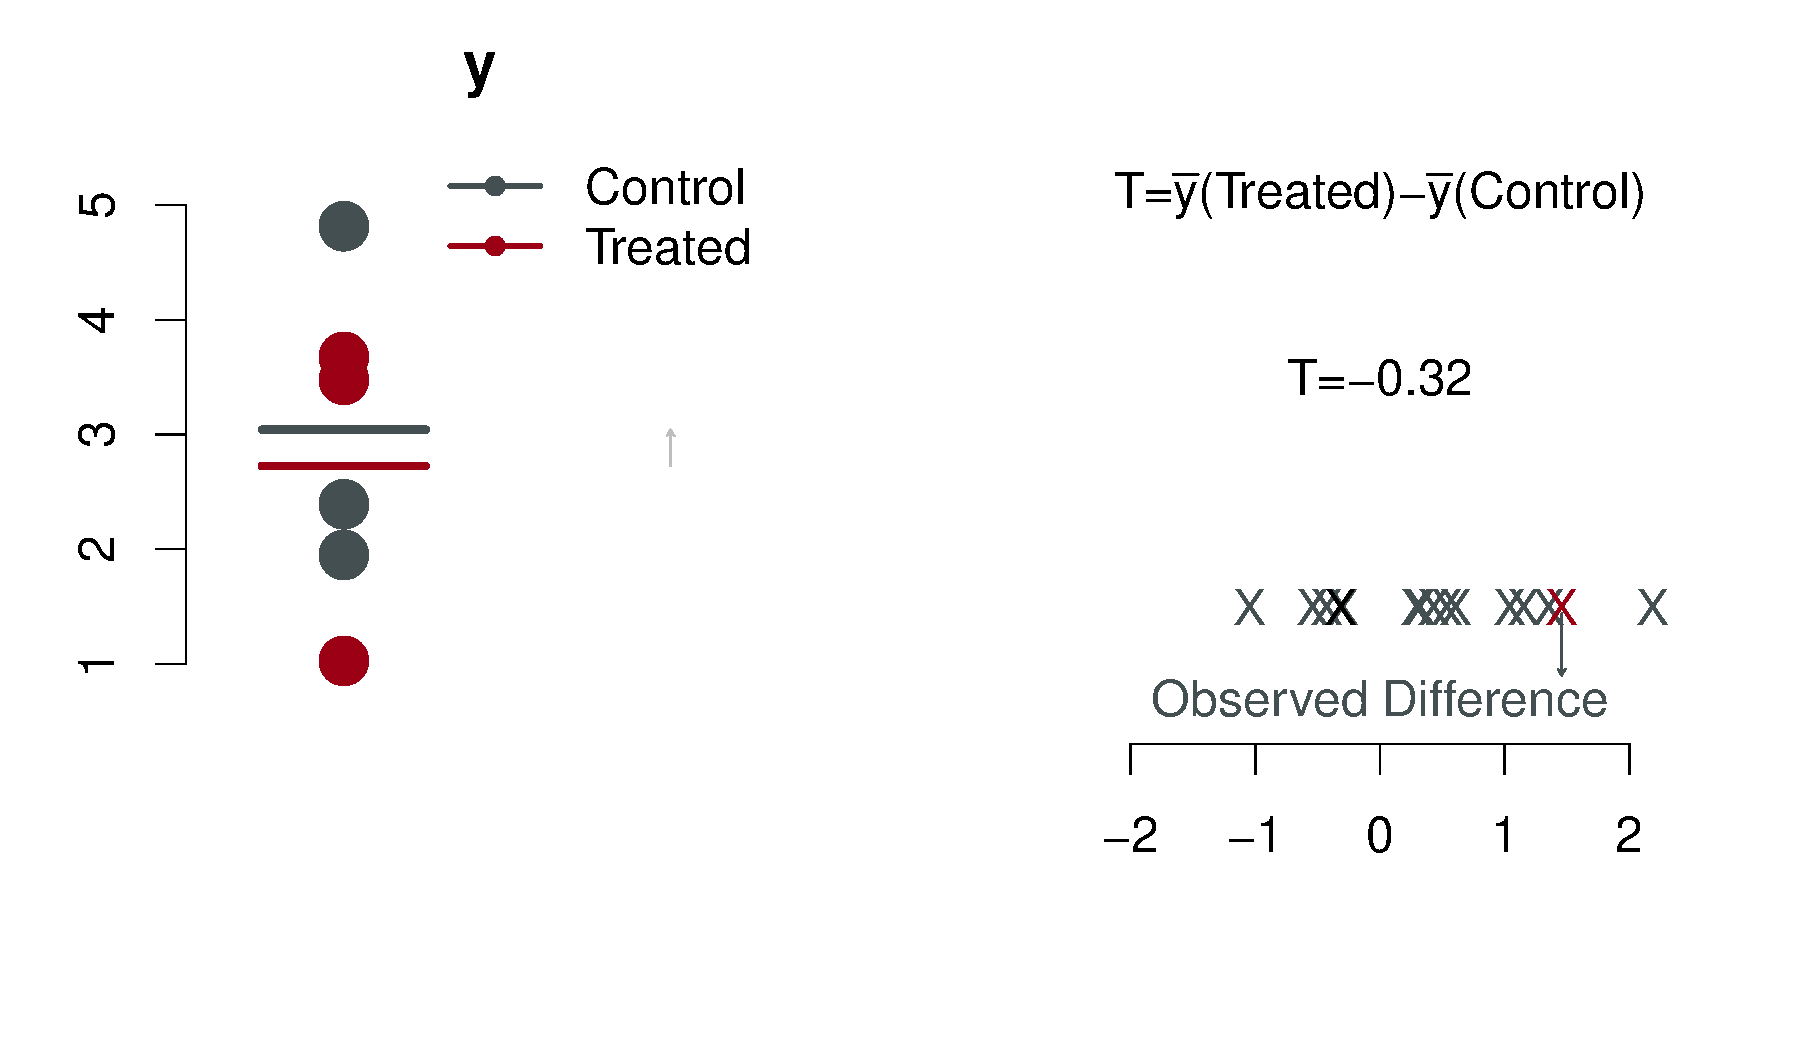
\includegraphics[width=1.1\textwidth]{figures/permsslides15} 
\end{center}
\end{frame}


\begin{frame}{A Naive approach to Permutation Testing}
 \ldots and go on with all hypothetical experiments\ldots 
\begin{center}
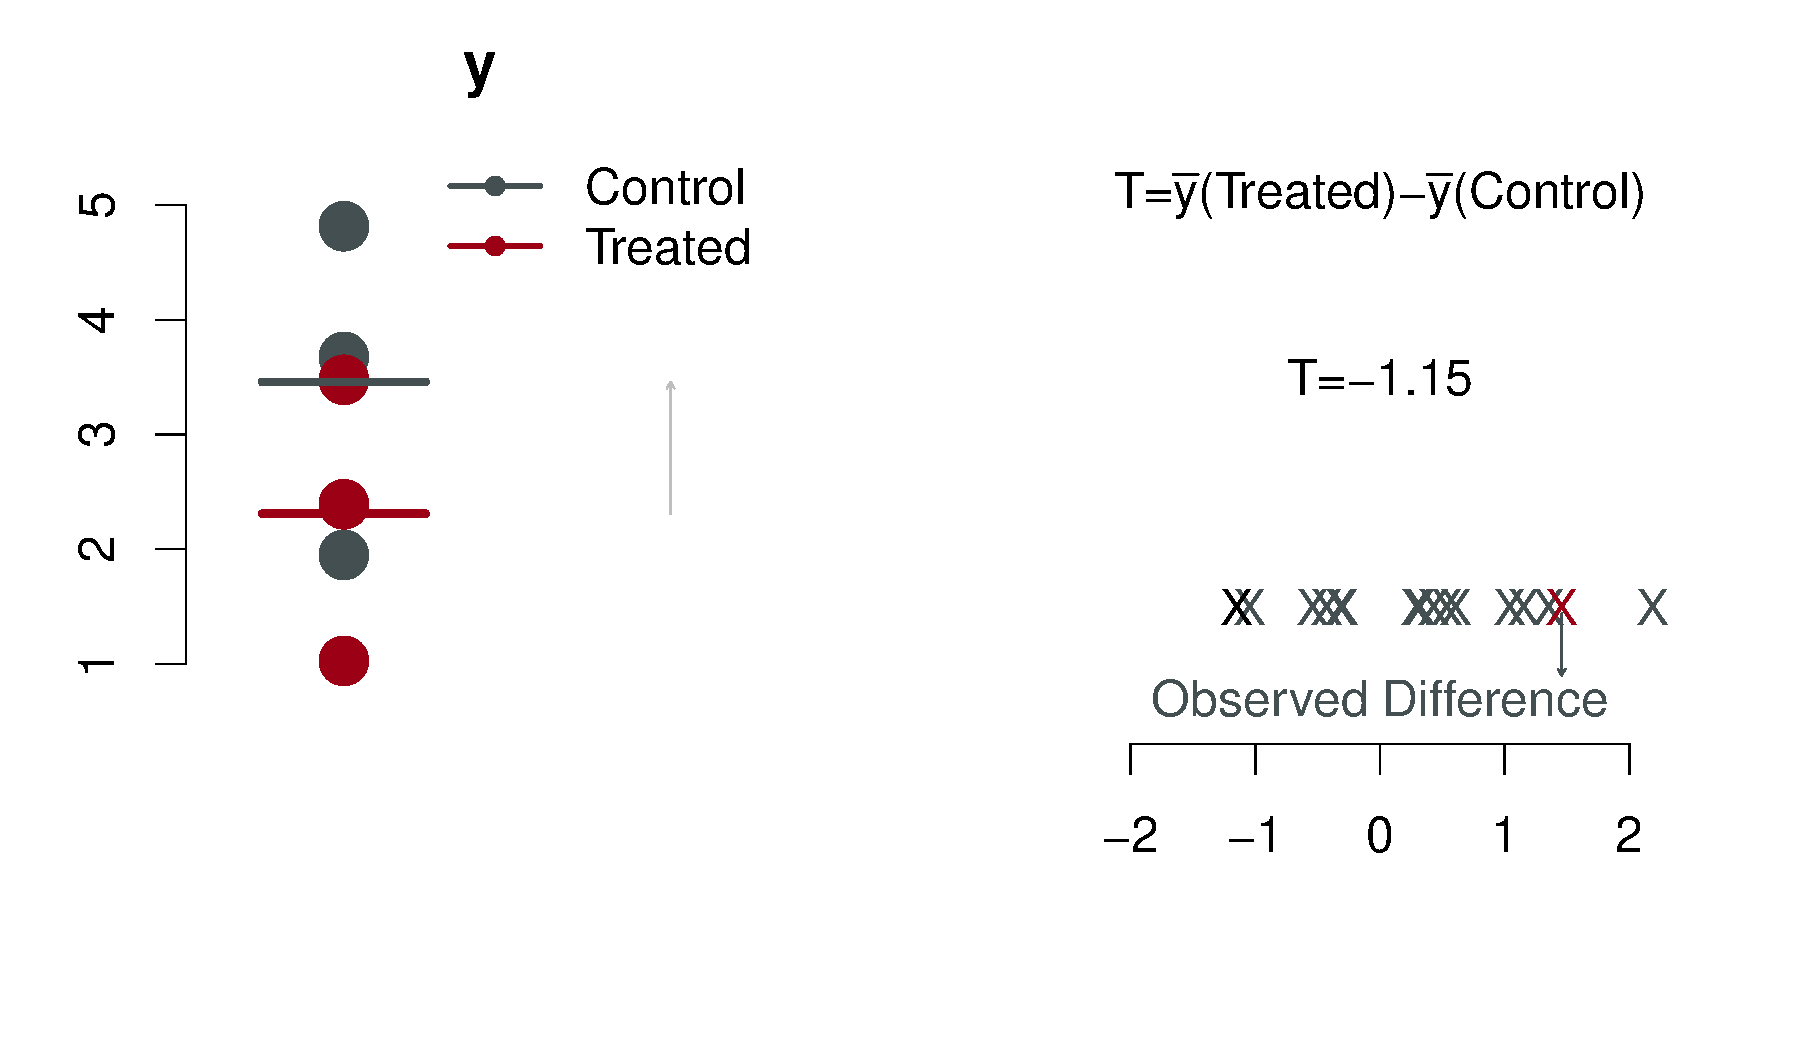
\includegraphics[width=1.1\textwidth]{figures/permsslides16} 
\end{center}
\end{frame}


\begin{frame}{A Naive approach to Permutation Testing}
 \ldots and go on with all hypothetical experiments\ldots 
\begin{center}
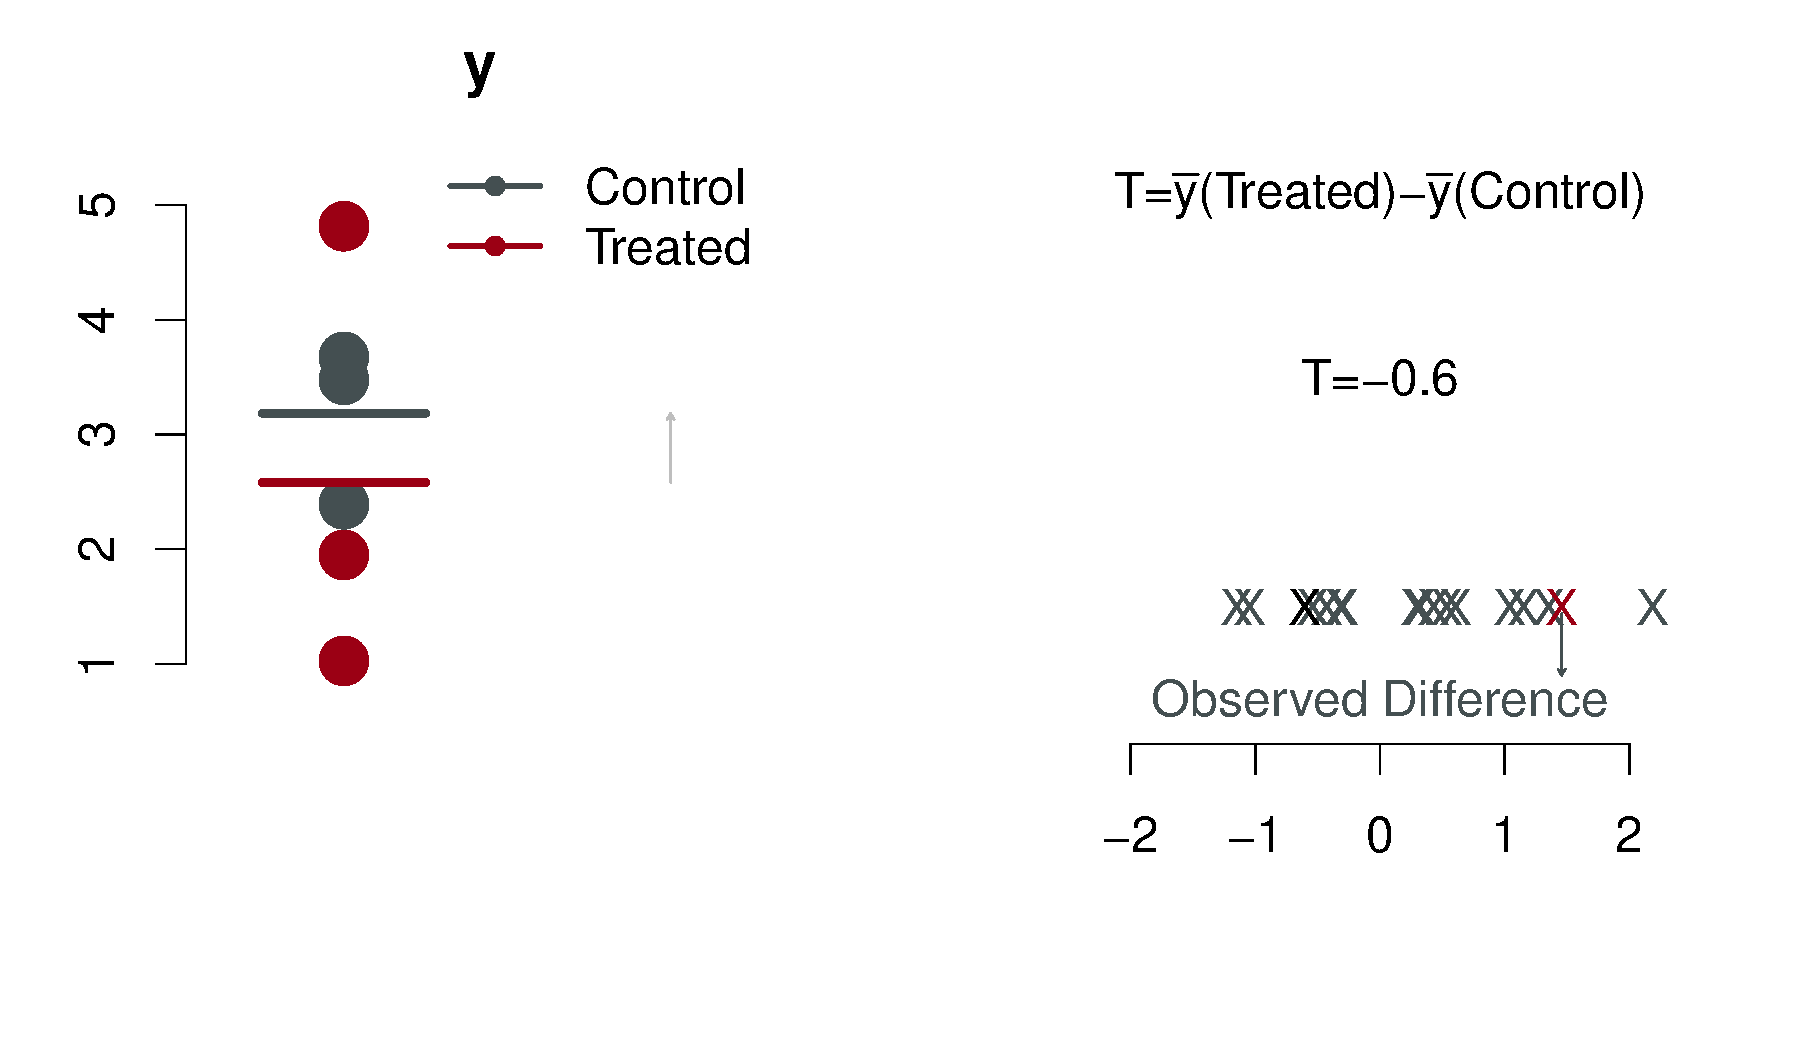
\includegraphics[width=1.1\textwidth]{figures/permsslides17} 
\end{center}
\end{frame}


\begin{frame}{A Naive approach to Permutation Testing}
 \ldots and go on with all hypothetical experiments\ldots 
\begin{center}
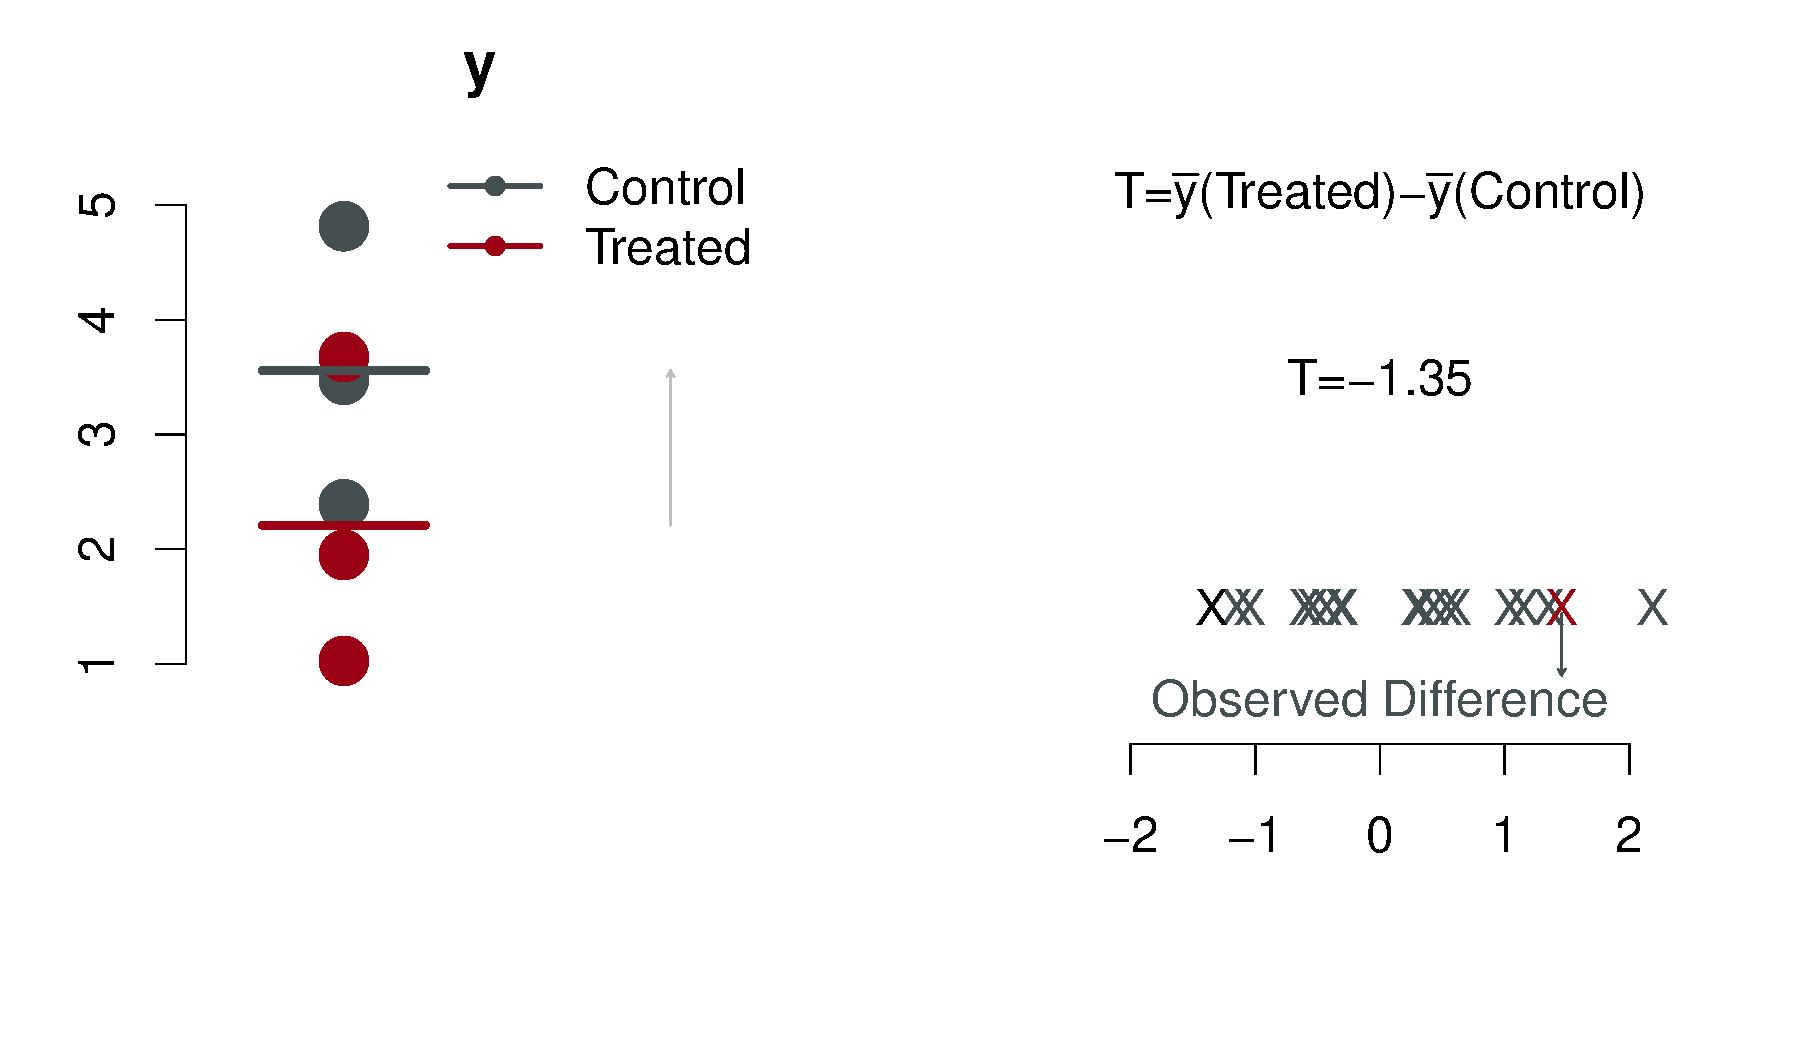
\includegraphics[width=1.1\textwidth]{figures/permsslides18} 
\end{center}
\end{frame}


\begin{frame}{A Naive approach to Permutation Testing}
 \ldots and go on with all hypothetical experiments\ldots 
\begin{center}
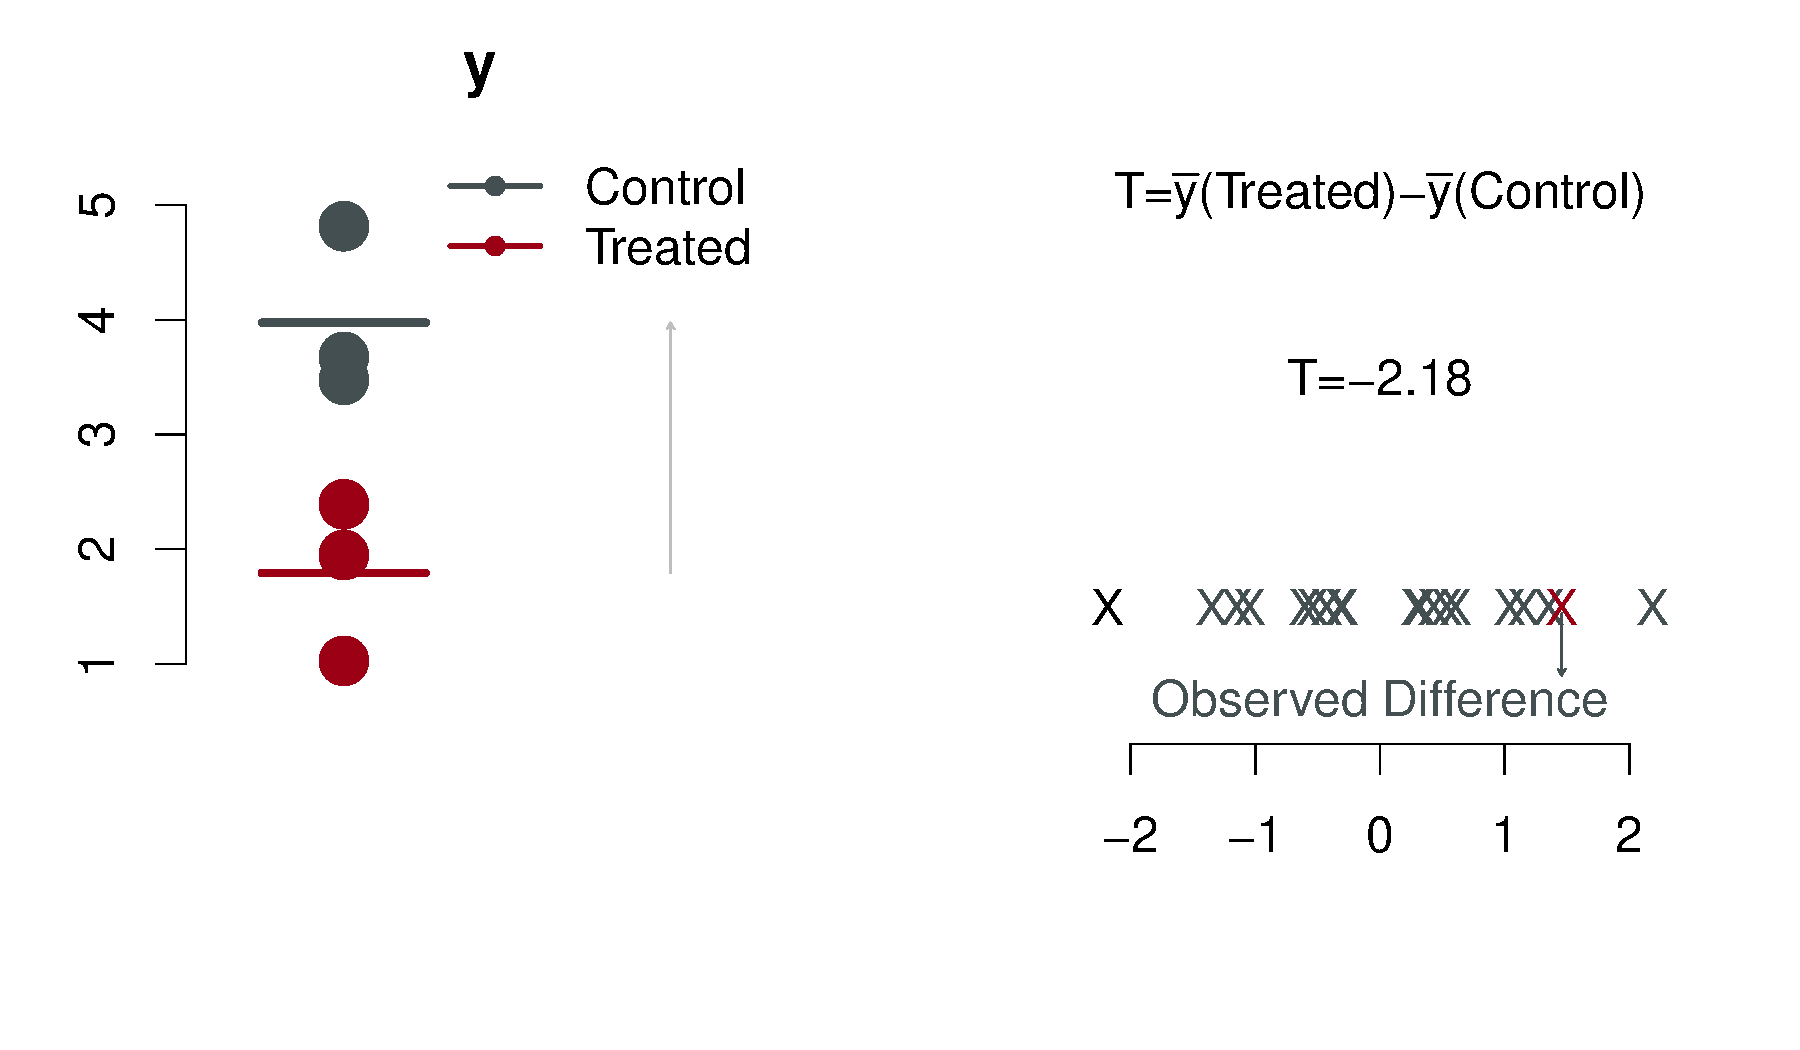
\includegraphics[width=1.1\textwidth]{figures/permsslides19} 
\end{center}
\end{frame}

\begin{frame}{A Naive approach to Permutation Testing}
 \ldots and compute the p-value!
\begin{center}
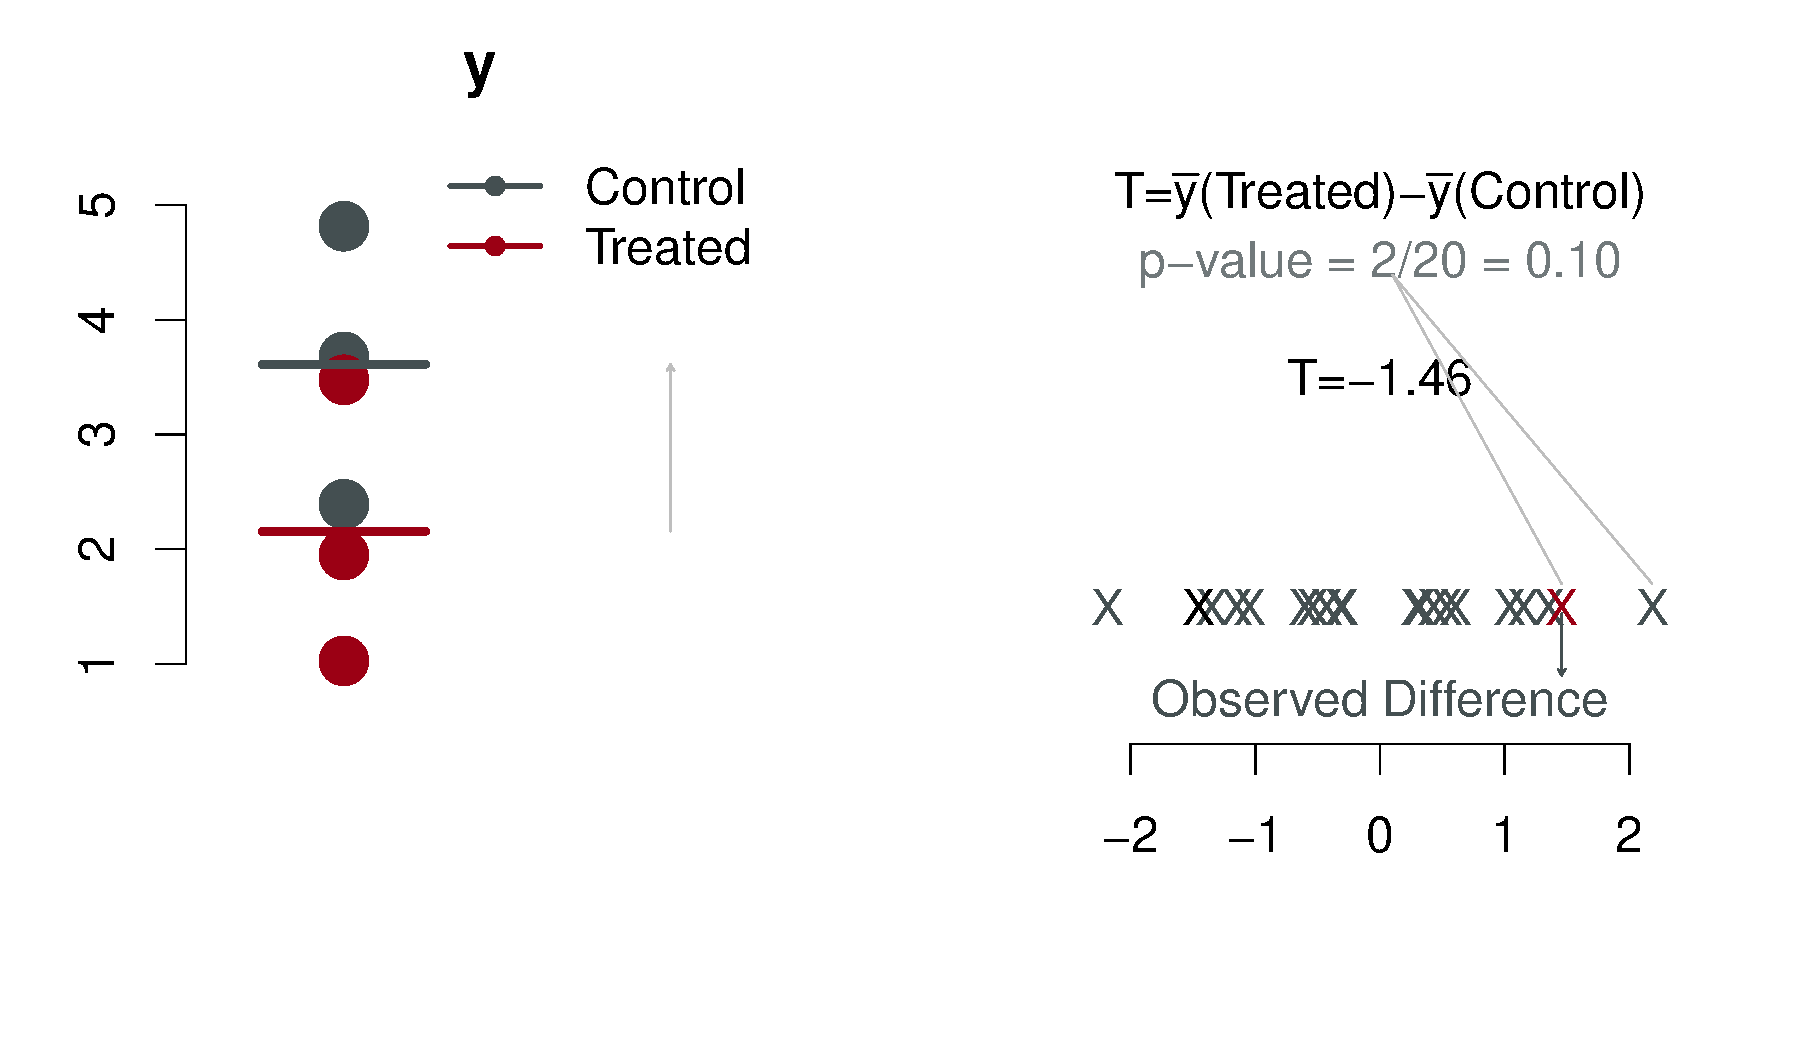
\includegraphics[width=1.1\textwidth]{figures/permsslides20} 
\end{center}
\end{frame}